%\documentclass[12pt]{amsart}
%\usepackage{geometry} % see geometry.pdf on how to lay out the page. There's lots.
%\usepackage{datetime}
%\usepackage{setspace}
%\usepackage{graphicx}
%\usepackage{caption}
%\usepackage{subcaption}
%\doublespacing
%\geometry{a4paper} % or letter or a5paper or ... etc
%\DeclareMathOperator*{\argmin}{argmin}

% See the ``Article customise'' template for come common customisations

%\title{Wind chapter}
%\author{Percy Link}
%\date{\currenttime  \today}

\chapter{Wind Chapter}
\label{c.wind}

Abstract.


%%% BEGIN DOCUMENT
%\begin{document}

%\maketitle


%\documentclass[12pt]{amsart}
%\usepackage{geometry} % see geometry.pdf on how to lay out the page. There's lots.
%\usepackage{datetime}
%\geometry{a4paper} % or letter or a5paper or ... etc
%% \geometry{landscape} % rotated page geometry
%
%% See the ``Article customise'' template for come common customisations
%
%\title{Wind chapter}
%\author{Percy Link}
%\date{\currenttime \ \today} % delete this line to display the current date
%
%%%% BEGIN DOCUMENT
%\begin{document}
%
%\maketitle

\section{Introduction}

In this chapter, we investigate the effect of changes in land surface heat fluxes, mediated by modifications in soil moisture, on near-surface winds in California.  Accurate understanding and simulation of near-surface winds is necessary for a range of applications, including water vapor and pollutant transport studies, weather forecasting, aviation, and wind energy forecasting.  Here, we focus on wind forecasting for wind energy applications and on winds at a specific wind farm, the Solano Wind Project in the Sacramento-San Joaquin River Delta region of California.  A regional atmospheric model is used to test the sensitivity of Solano winds to different regions' soil moisture and to quantify the magnitude of the effect at different times of day across a range of soil moisture changes.  We demonstrate that accurate soil moisture information can improve wind forecasts.  This study serves as a prototype for characterizing the importance of soil moisture information for wind forecasts at other wind farms.

Accurate wind forecasts can reduce the cost of integrating wind energy into the electric grid on a large scale.  In order to reduce CO$_2$ emissions to the degree necessary to avert dangerous climate change [\cite{stocker2013ipcc}], electric utilities will need to transition to non-fossil-fuel energy sources, including a large fraction of wind energy [\cite{jacobson2011providing}].  However, although wind energy has large peak generation potential, it is intermittent, and the instantaneous mismatch between wind generation and electric demand must be met with other generation.  In most utilities, allocations of conventional electric generation (coal, natural gas, hydroelectric, and nuclear) are made one day in advance, based on forecasted net demand (demand minus wind and solar supply).  At shorter lead times (hour-ahead to real-time), imbalances between the day-ahead allocations of conventional generation and the actual net demand must be met with, in the case of a shortfall, more expensive quick-startup generation, or in the case of excess generation, wasted energy resources.  These imbalance costs add significantly to the cost of wind energy (around 10\% of a wind generator's income in a liberalized market [\cite{fabbri2005assessment}]).  Improved accuracy of wind forecasts could reduce imbalance costs, making integration of wind into the electric grid more economically feasible: wind and solar forecasting could reduce energy costs by \$0.01 to \$0.02 per kWh at 30\% wind and solar penetration [\cite{energy2010western}], or 8-15\% of the average US cost of electricity (\$0.13/kWh in July 2014 [\cite{eia2014}]).

%; and at high wind penetration, \$68 million to \$160 million could be saved annually in California using current state of the art forecasting, with an opportunity to save \$19 million to \$38 million more with forecast accuracy improvements [Porter and Rogers, 2010].

The major wind forecasting companies in North America and Europe use numerical weather prediction (NWP) models to make their day-ahead forecasts, often in combination with statistical post-processing [\cite{porter2010status}; \cite{foley2012current}; \cite{monteiro2009wind}].  NWP models simulate atmospheric wind speed, temperature, pressure, and humidity (among other variables) by solving the equations for conservation of momentum, mass, and energy, discretized in three spatial dimensions and in time.  NWP models require bottom boundary fluxes of energy, moisture, and momentum, but little attention has been paid to these bottom boundary fluxes in the wind energy literature (with the notable exceptions of \cite{marjanovic2014} and \cite{wharton2011review}, discussed below).  Wind energy forecast research has concentrated instead on sensitivity to NWP physical parameterizations, especially planetary boundary layer (PBL) schemes [\cite{draxl2014evaluating}; \cite{marjanovic2014}], and to grid resolution [\cite{marjanovic2014}, \cite{carvalho2012sensitivity}].  There have also been extensive efforts to enhance NWP wind energy forecasts by running model ensembles [\cite{deppe2013wrf}; \cite{pinson2009ensemble}] and by applying various model output statistics (MOS) algorithms [\cite{bedard2013development}; \cite{ranaboldo2013implementation}; \cite{ellis2014predicting}; \cite{ortiz2011short}; \cite{kusiak2009wind}].

%The prediction of ramps (rapid increases or decreases in wind power) remains a challenge [Carcangiu \textit{et al.}, 2014; Ellis \textit{et al.}, 2014; Wharton \textit{et al.}, 2011].

%Regional NWP models require boundary condition information at the lateral boundaries of the grid, as well as bottom boundary fluxes of energy, moisture, and momentum.  If the bottom boundary is land, these fluxes are usually calculated with a land surface model.  

%Wind energy forecasts are sensitive to NWP model resolution and physical parameterizations, especially planetary boundary layer (PBL) schemes [Draxl \textit{et al.}, 2014; Marjanovic \textit{et al.}, 2014]; the optimal PBL scheme depends in part on atmospheric stability conditions [Draxl \textit{et al.}, 2014; Marjanovic \textit{et al.}, 2014], and the optimal grid resolution depends largely on terrain complexity, with more complex terrain requiring higher resolution [Marjanovic \textit{et al.}, 2014, Carvalho \textit{et al.}, 2012].  Ensembles of NWP runs have been used to characterize a forecast probability distribution [Deppe \textit{et al.}, 2013; Pinson and Madsen, 2009].  Various model output statistics (MOS) algorithms incorporating historical observations have been shown to improve NWP forecasts in post-processing; in particular, machine learning algorithms such as directional multipoint linear regression [B\'edard \textit{et al.}, 2013], multiple linear regression [Ranaboldo \textit{et al.}, 2013], random forests, generalized linear models, gradient boosting, and support vector machines [Ellis \textit{et al.}, 2014; Ortiz-Garc\'ia \textit{et al.}, 2011], and neural networks [Kusiak \textit{et al.}, 2009] have shown promise.  The prediction of ramps (rapid increases or decreases in wind power) remains a challenge [Carcangiu \textit{et al.}, 2014; Ellis \textit{et al.}, 2014; Wharton \textit{et al.}, 2011].

The influence of soil moisture and land surface heating on wind prediction has received little attention in the wind energy forecasting literature, even though fluxes of energy at the land surface are known to influence regional circulations.  Soil moisture heterogeneity, and the resulting contrasts in sensible heat flux, can drive mesoscale circulations on land with wind speeds of several m/s [\cite{chen1994impact}; \cite{avissar1998evaluation}].  Thermal contrast between land and ocean can drive sea-breeze circulations with wind speeds up to 10 m/s [\cite{miller2003sea}], and the strength of the thermal contrast and of the resulting wind depends in part on soil moisture because of its influence on land surface temperature [\cite{physick1980numerical}].  In one of the few wind energy papers to discuss the effect of soil moisture on wind forecasts, \cite{marjanovic2014} show that the forecast at a California wind farm is sensitive to initial soil moisture, and in a related study, \cite{wharton2011review} show that soil moisture can be important for forecasting wind ramps, which remain a challenge in wind energy forecasting [\cite{carcangiu2013wind}; \cite{ellis2014predicting}].

California low-level winds are strongly influenced by the contrast of land surface heating with the adjacent cool ocean [\cite{zhong2004diurnal}], and as such, winds at the Solano wind farm are likely to depend on soil moisture.  Solano sits in a valley pass between the ocean and California's Central Valley (Figure \ref{fig:windSol_domainmap}, red star), and onshore winds are channeled and accelerated through the pass; this topographic channeling also constrains the wind direction at low levels near Solano to remain near-westerly [\cite{zhong2004diurnal}; \cite{mansbach2010synoptic}].  The diurnal cycle of land surface heating drives a marked diurnal cycle in wind speed in the Solano area, with minimum wind speeds in the morning and maximum speeds in the late afternoon and evening [\cite{zhong2004diurnal}; \cite{mansbach2010synoptic}].  Additionally, the strongest winds occur in the summer at Solano, in part due to generally stable synoptic conditions created by the north Pacific summertime high pressure that allow the strong surface temperature contrast between ocean and land to drive onshore flow [\cite{zhong2004diurnal}; \cite{mansbach2010synoptic}]. Because land surface heating is important for generating winds at Solano, it is likely that errors in soil moisture initial conditions will create errors in NWP wind forecasts.

In this work, we seek to understand the sensitivity of Solano wind to soil moisture, and the physical mechanism underlying the sensitivity.  We investigate the following questions:
\begin{itemize}
\item Which region's soil moisture has the maximum impact on wind speed at Solano?
\item At what time of day is Solano wind most sensitive to soil moisture?  What changes in the amplitude and timing of the wind diurnal cycle result from changes in soil moisture?
\item How do wind forecast errors scale with soil moisture changes/errors?  Are there particular ranges of soil moisture where wind forecasts are particularly sensitive?
\item What is the physical mechanism for soil moisture's influence on Solano winds?
\end{itemize}

To answer these questions, we conduct numerical experiments with a regional atmospheric model commonly used in wind energy forecasting research.  We perturb soil moisture in different California regions and to different degrees, and we quantify the response of Solano turbine-level wind magnitude and timing.  Moreover, we identify regions where pressure correlates with Solano wind and relate pressure changes to changes in surface heating; and we attribute changes in wind to changes in the terms of the momentum budget.

%The model is an imperfect representation of the world; it captures many of the important processes, but we do not contend that it represents land surface fluxes perfectly.  In this study, we both investigate the real-world physical sensitivity of the winds to soil moisture, to the degree possible given the model errors, and also characterize the sensitivity within the model itself.  Even if the internal model sensitivity is not fully realistic, this tool is in common usage in wind energy forecasting, and thus it is important to understand the sensitivity of the tool to the inputs.


%\end{document}


%\documentclass[12pt]{amsart}
%\usepackage{geometry} % see geometry.pdf on how to lay out the page. There's lots.
%\usepackage{datetime}
%\usepackage{setspace}
%\doublespacing
%\geometry{a4paper} % or letter or a5paper or ... etc
%% \geometry{landscape} % rotated page geometry
%
%% See the ``Article customise'' template for come common customisations
%
%\title{Wind chapter}
%\author{Percy Link}
%\date{\currenttime \ \today} % delete this line to display the current date
%
%%%% BEGIN DOCUMENT
%\begin{document}
%
%\maketitle

\section{Methods}

The sensitivity of Solano wind forecasts to soil moisture is tested using numerical experiments with a regional atmospheric model, the Weather Research and Forecasting (WRF) model.  The WRF model, described in Section \ref{sec:BL_WRFdesc} and in detail in Skamarock et al. [2008], is a three-dimensional, non-hydrostatic regional atmospheric model with terrain-following vertical coordinates. WRF has been used extensively in wind energy forecasting [CITATIONS], with generally good performance [CITATIONS, METRIC].  Accuracy of WRF-forecasted turbine-level winds depends on \textit{(resolution, PBL scheme, lateral forcing, soil moisture **)} [CITATIONS].

\subsection{Model setup}

We run WRF with two nested domains centered on the Solano wind farm (Figure \ref{fig:windSol_domainmap}); the domains are described in Table \ref{table:windSol_domains}.  As in Chapter XX, the outer grid forces the lateral boundaries of the inner grid, and the inner grid feeds back to the outer grid across the region where the two domains overlap [Skamarock et al., 2008].  The outer and inner domain are Arakawa-C grids with horizontal resolution of 8.1 km and 2.7 km, respectively; preliminary tests with a third finer grid (0.9 km) showed little change in the forecasted winds, similar to the results of Marjanovic \textit{et al.} [2014], who found little accuracy improvement with horizontal resolution below 2.7 km in their simple terrain case.  The domain has 45 vertical levels, with a minimum spacing of $\sim$30 m near the surface and increasing with height, interpolated quadratically by the log of pressure (the default WRF setting); turbine-level (60-100 m) wind forecasts are not very sensitive to vertical resolution beyond about 40 levels with this vertical interpolation scheme in WRF [Marjanovic \textit{et al.}, 2014, and references therein].

\begin{figure}[here]
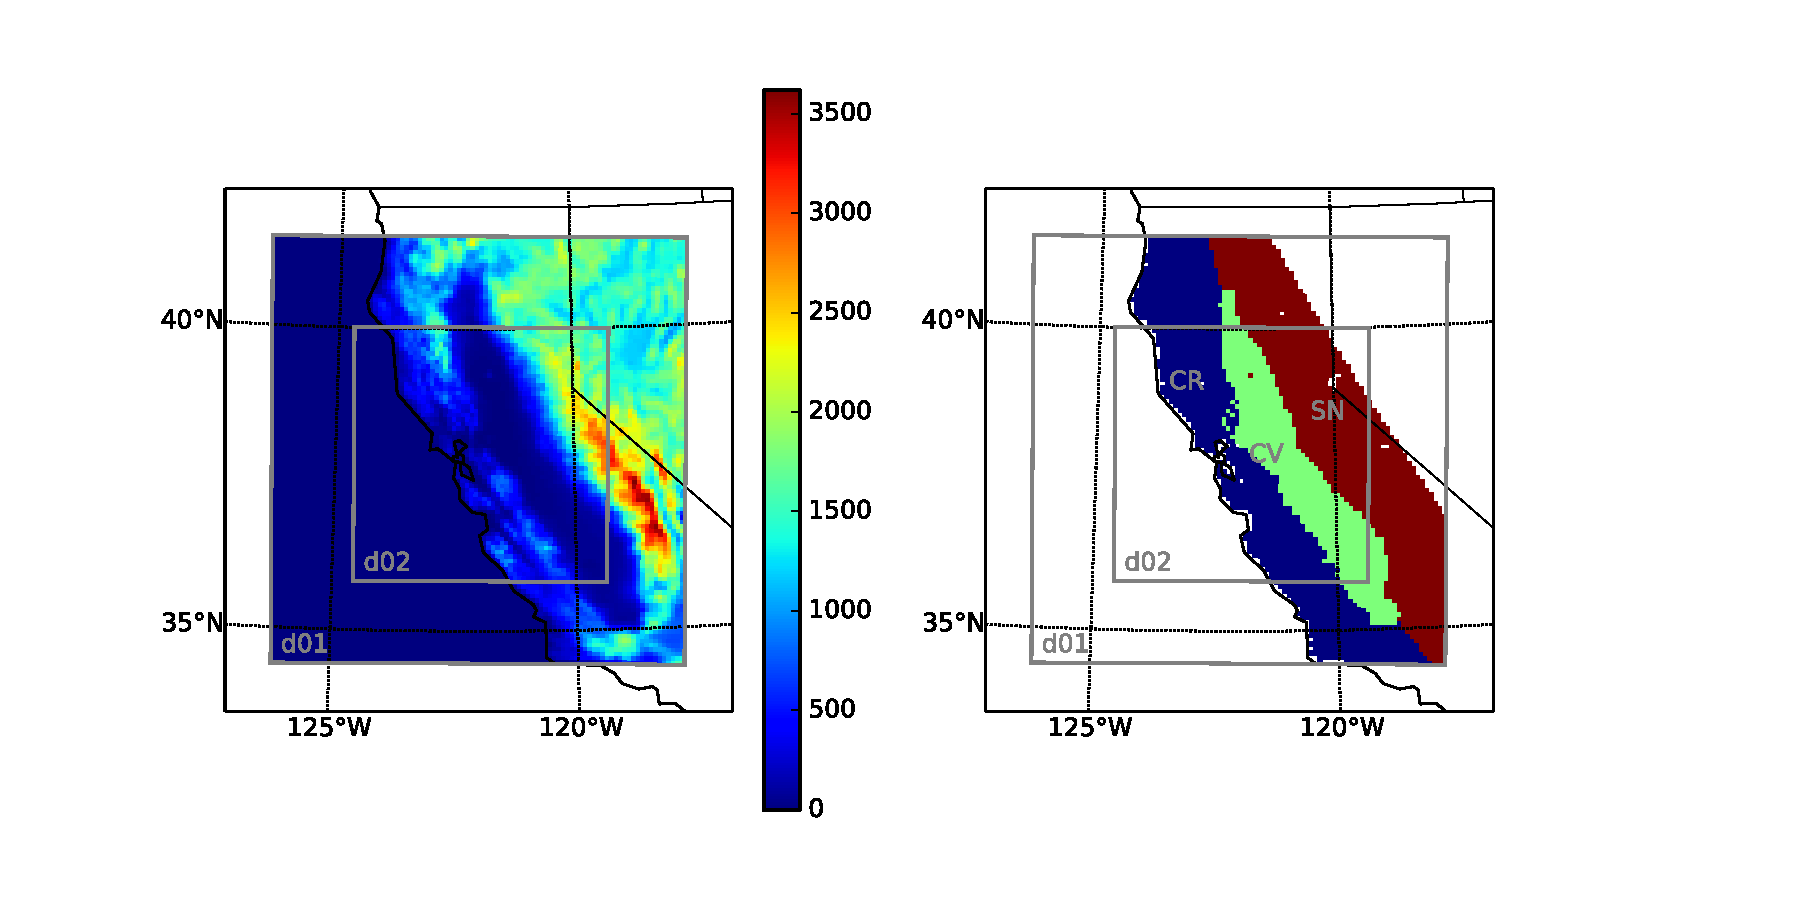
\includegraphics[width=1\textwidth]{ch3-wind/img/domain_map.pdf}
\caption{WRF model domains, showing (a) topographic height in m, and (b) regions used for soil moisture experiments in this study: the Coast Range (CR, blue), Central Valley (CV, green), and Sierra Nevada (SN, red). d01 refers to the outer model domain, and d02 refers to the inner domain.}
\label{fig:windSol_domainmap}
\end{figure}

\begin{table}
\begin{tabular}{ l c c c c c c c }
\hline
Domain & $\Delta x$ (km) & $\Delta y$ (km) & $nx$ & $ny$ & $nz$ & $\Delta t$ (s) & USGS data res \\ \hline
d01 & 8.1 & 8.1 & 96 & 99 & 45 & 45 & 2 min\\
d02 & 2.7 & 2.7 & 175 & 175 & 45 & 15 & 2 min\\
\hline
\end{tabular}
\caption{Model domains. d01 refers to the outer domain, and d02 refers to the inner domain.}
\label{table:windSol_domains}
\end{table}

In WRF, the atmospheric model is coupled to the Noah land surface model with USGS land use and soil classifications [Skamarock \textit{et al.}, 2008].  The observed distributions of land use and soil types are used, as are the default vegetation water-use parameters for each land use type [REFS], in order to simulate as closely as possible the real present day sensitivity of Solano winds to soil moisture.  Uncertainties associated with errors in the model representation of water movement in the subsurface and plant water use are addressed in the Discussion. 

As in Chapter XX, the ACM2 PBL scheme is used, following the recommendations of Marjanovic \textit{et al.} [2014] for a locally forced simple terrain case in California; this PBL scheme includes both local (small-scale turbulent) and nonlocal (large convective plume) vertical transport, and can thus simulate both stable and unstable conditions [Pleim, \textit{2007}] A LITTLE MORE DETAIL ABOUT THE PHYSICS.  The model is forced at the lateral boundaries with NCEP Eta 212 grid (40 km) operational analysis [NCEP, 1998].  Other parameterization schemes and settings are the same as those in Chapter XX Table XX.  Model variables are output every 30 minutes.

All experiments are run for the period 2009-06-26 00:00 UTC to 2009-07-11 00:00 UTC, and the first 32 hours are discarded as model spin-up.  This period was chosen for several reasons: (1) it contains a range of synoptic conditions (weak background wind June 27-July 5, and strong background wind July 6-11), (2) turbine-level wind speeds in this region are highest in the spring and summer [Zhong \textit{et al.}, 2004; Mansbach, 2010], and (3) the sensitivity to soil moisture is expected to be strongest in the warm season when radiation incident to the land surface is greatest, because changes in the relative partitioning between evapotranspiration and sensible heat flux have the largest absolute magnitude then.

\subsection{Soil moisture experiments}

The model experiments are listed in Table \ref{table:windSol_runlist}.  In the first set of experiments, we test the sensitivity of Solano winds to soil moisture in different large-scale regions of California.  In cases dryCR, dryCV, and drySN, the background volumetric soil moisture (model variable SMOIS, m$^3$ water/m$^3$ total volume) is set to 0.25, and the soil moisture of the test region (respectively, the Coast Range, Central Valley, and Sierra Nevada, shown in Figure \ref{fig:windSol_domainmap}b) is set to 0.1.  These test cases are compared with a control case where all land has soil moisture of 0.25.  In cases wetCR, wetCV, and wetSN, the background soil moisture is set to 0.1, and the soil moisture of the test region is set to 0.25.  These test cases are compared with a control case where all land has soil moisture of 0.1.

The next set of experiments tests how the Solano wind response scales with soil moisture in the Central Valley, with a normal-to-wet background in the Coast Range and Sierra Nevada.  In cases CVXX (where XX is a numeric value), the Coast Range and Sierra Nevada regions' soil moisture is set to 0.2, and the Central Valley soil moisture is set to the value specified by XX.  These test cases are compared with a control case where all land has soil moisture of 0.2.
%In cases CVXXdry, the Coast Range and Sierra Nevada regions' soil moisture is set to 0.1, and the Central Valley soil moisture again is specified by XX.

In all cases, the soil moisture is set to the prescribed values at the model start time (2009-06-26 00:00 UTC) and is reset to the prescribed value each day at 08:00 UTC (midnight Pacific Standard Time); the soil moisture evolves according to the land surface model each day between resets.  The change in soil moisture between resets is small (up to 0.02 m$^3$/m$^3$ in the regional average when soils are wet and much less when soils are dry.  Additionally, the synoptic forcing, measured by wind speed at 500 hPa, varies little between the model runs (Figure XX), and synoptic winds are weak on June 27 to July 5 and strong on July 6 to 11.  In all three regions, land surface sensible heat flux is approximately 200 W/m$^2$ greater at midday with wet soil moisture (0.25) than dry soil moisture (0.1).  \textbf{Need to make figure showing these.}

%\begin{figure}[here]
%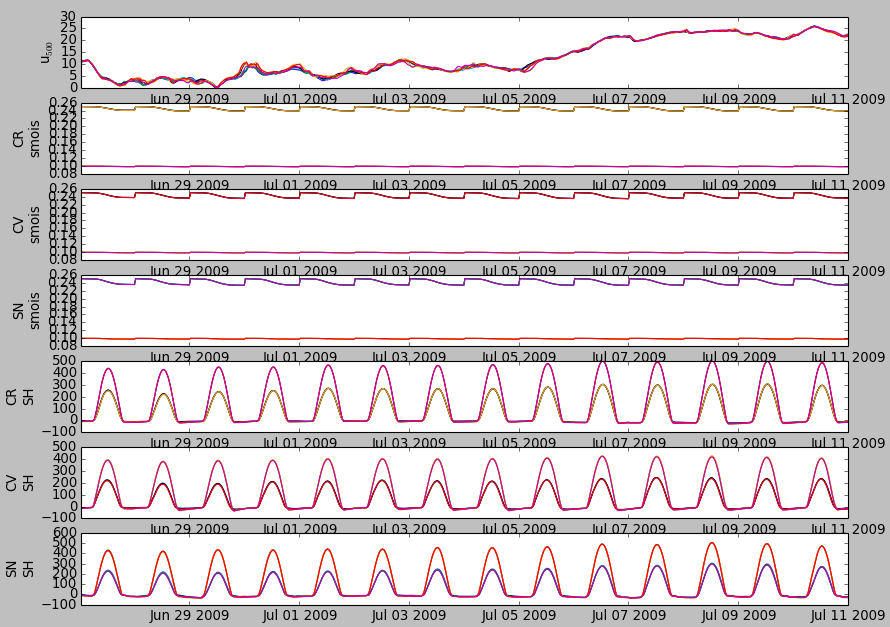
\includegraphics[width=1\textwidth]{ch3-wind/img/forcings_combo_good.png}
%\caption{Model forcing for all of the regional perturbation cases.  \textbf{I NEED ADVICE ON HOW TO DISPLAY THIS INFORMATION MORE CLEARLY AND/OR CONCISELY. Obviously, I need a legend for which color means which run.}  Top panel: wind speed over Solano at 500 hPa.  Panels 2-4: average soil moisture in the top soil layer for the CR region (panel 2), the CV region (panel 3), and the SN region (panel 4).  Panels 5-7: average surface sensible heat flux for the CR region (panel 5), the CV region (panel 6), and the SN region (panel 7).}
%\label{fig:windSol_forcings}
%\end{figure}

\begin{table}
\begin{tabular}{p{2.5cm} l p{3cm} p{3cm} p{3.5cm}}
\hline
Experiment & Run name & Background SMOIS (kg/kg) & Perturbed SMOIS region & Perturbed SMOIS value (kg/kg) \\
\hline
1 & CA-0.1 & 0.1 & none & n/a \\
1 & wetCR & 0.1 & Coast Range & 0.25 \\
1 & wetCV & 0.1 & Central Valley & 0.25 \\
1 & wetSN & 0.1 & Sierra Nevada & 0.25 \\
2 & CA-0.2 & 0.2 & none & n/a \\
2 & dryCR & 0.25 & Coast Range & 0.1 \\
2 & dryCV & 0.25 & Central Valley & 0.1 \\
2 & drySN & 0.25 & Sierra Nevada & 0.1 \\
3 & CA-0.25 & 0.25 & none & n/a \\
3 & CV0.05 & 0.2 & Central Valley & 0.05 \\
3 & CV0.1 & 0.2 & Central Valley & 0.1 \\
3 & CV0.15 & 0.2 & Central Valley & 0.15 \\
3 & CV0.25 & 0.2 & Central Valley & 0.25 \\
3 & CV0.3 & 0.2 & Central Valley & 0.3 \\
3 & CV0.35 & 0.2 & Central Valley & 0.35 \\
%CV0.05dry & 0.1 & Central Valley & 0.05 \\
%CV0.15dry & 0.1 & Central Valley & 0.15 \\
%CV0.2dry & 0.1 & Central Valley & 0.2 \\
%CV0.25dry & 0.1 & Central Valley & 0.25 \\
%CV0.3dry & 0.1 & Central Valley & 0.3 \\
%CV0.35dry & 0.1 & Central Valley & 0.35 \\
\hline
\end{tabular}
\caption{Model experiments: (1) Dry background, wet perturbation region; (2) Wet background, dry perturbation region; (3) Sensitivity to Central Valley soil moisture.}
\label{table:windSol_runlist}
\end{table}

%\end{document}


%\documentclass[12pt]{amsart}
%\usepackage{geometry} % see geometry.pdf on how to lay out the page. There's lots.
%\usepackage{datetime}
%\usepackage{setspace}
%\doublespacing
%\geometry{a4paper} % or letter or a5paper or ... etc
%% \geometry{landscape} % rotated page geometry
%
%% See the ``Article customise'' template for come common customisations
%
%\title{Wind chapter}
%\author{Percy Link}
%\date{\currenttime \ \today} % delete this line to display the current date
%
%%%% BEGIN DOCUMENT
%\begin{document}
%
%\maketitle

\section{Results}

We first characterize the differences in Solano turbine-level wind resulting from the soil moisture tests (Section \ref{subsec:CharWindChanges}).  We then investigate the physical mechanism linking changes in soil moisture to changes in Solano wind timing and magnitude (Section \ref{subsec:PhysMech}).

\subsection{Characterization of Solano wind sensitivity to soil moisture}
\label{subsec:CharWindChanges}

\subsubsection{California low-level wind system}
\label{subsubsec:control_winds}

%Before presenting the Solano winds, we quantify the synoptic and land-surface-heating forcing in each case, and we characterize the control case winds.  The synoptic forcing, measured by wind speed at 500 hPa, varies little between the model runs (Figure \ref{fig:windSol_forcings}), and synoptic winds are weak on June 27 to July 5 and strong on July 6 to 11.  In all three regions, land surface sensible heat flux is approximately 200 W/m$^2$ greater at midday with wet soil moisture (0.25) than dry soil moisture (0.1).

The low-level winds in California follow a strong diurnal cycle, driven by the diurnal cycle of the temperature difference and thus the pressure difference between land and ocean.  Regional low-level winds in the control case are consistent with previous studies of California surface winds (Figure \ref{fig:windSol_WindMapsRg} first column, Zhong \textit{et al.}, 2004; Mansbach, 2010); flow is strong through the Solano pass and splits into northward and southward branches in the Central Valley.  The southward branch is stronger than the northward branch at 06:00 and 14:00, and the northward branch strengthens at 18:00 and 00:00.  The pressure gradient from the San Francisco Bay to the Central Valley remains strong from 14:00 to 00:00 and weakens by 06:00.  \textbf{Note: I need to remake these plots to label the pressure change contours.}

\begin{figure}[here]
\includegraphics[angle=90,origin=c,width=1\textwidth]{ch3-wind/img/wind_map_regions2.eps}
\caption{Wind speed (color shading) and direction (vectors) and pressure (color contours) at 110 m ASL on the d02 domain, averaged by hour over the two-week runs.  (a)-(d) CA-0.25 control case.  (e)-(h) dryCR case, changes in wind and pressure.  (i)-(l) dryCV case, changes in wind and pressure.  (m)-(p) drySN case, changes in wind and pressure.  Top row: average for hour 06:00 for the whole run; second row: average for hour 14:00; third row: average for hour 18:00; bottom row: average for hour 00:00.}
\label{fig:windSol_WindMapsRg}
\end{figure}

\begin{figure}[here]
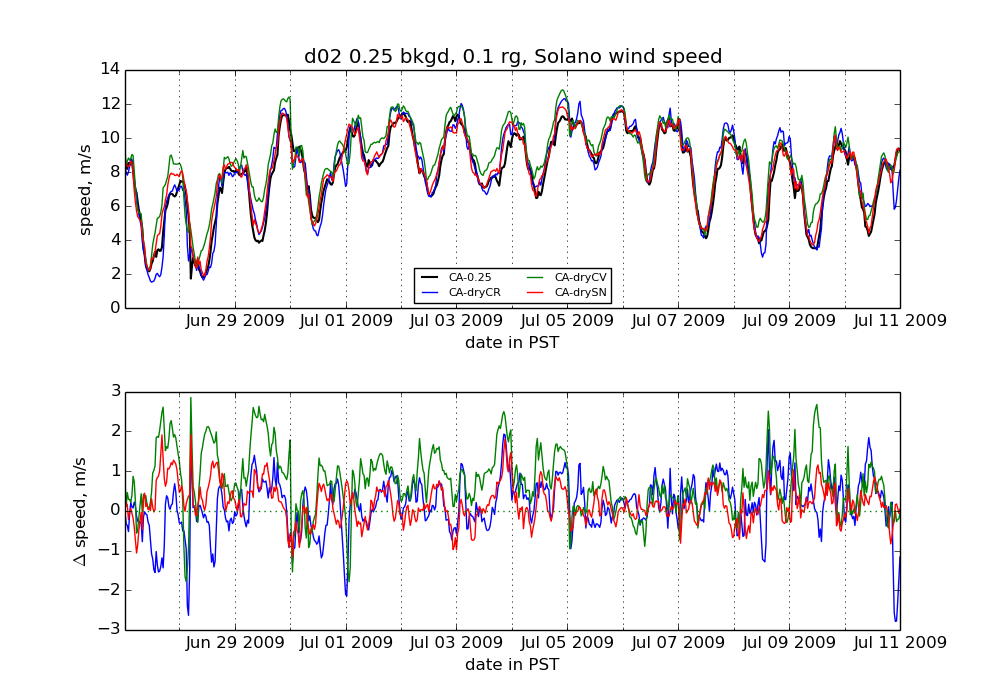
\includegraphics[width=1\textwidth]{ch3-wind/img/solano_wind_wetbkd_dryrg_d02_level0.png}
\caption{Time series of wind speed magnitude at 60 m AGL for the d02 grid point nearest the Solano wind farm, for the wet background and dry perturbation tests.  The model spin-up period is excluded.}
\label{fig:windSol_TseriesDryRg}
\end{figure}

\begin{figure}[here]
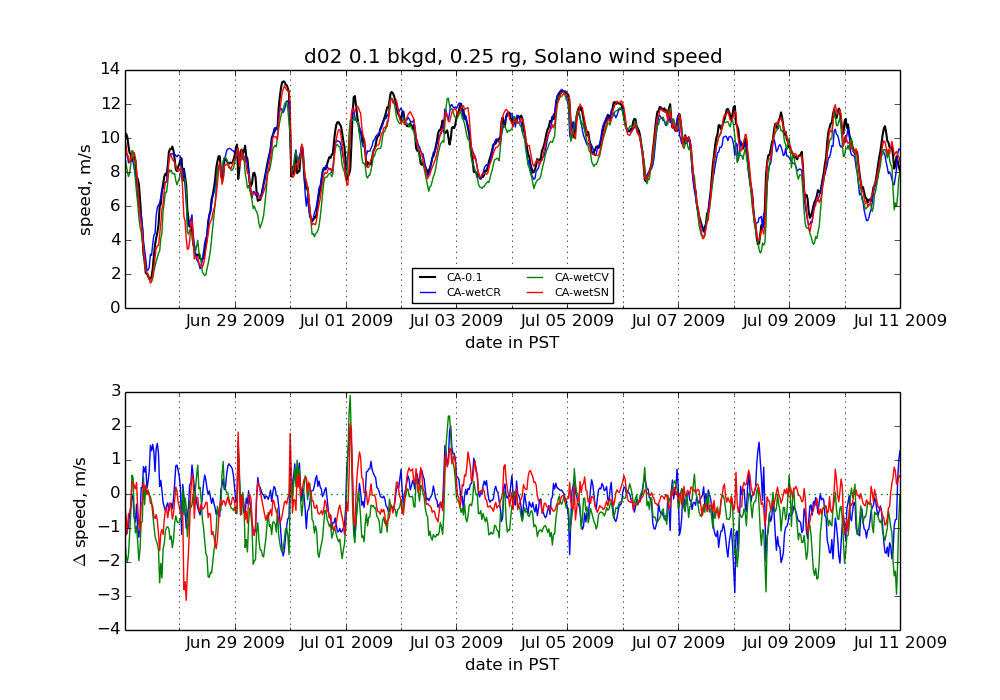
\includegraphics[width=1\textwidth]{ch3-wind/img/solano_wind_drybkd_wetrg_d02_level0.png}
\caption{Time series of wind speed magnitude at 60 m AGL for the d02 grid point nearest the Solano wind farm, for the dry background and wet perturbation tests.  The model spin-up period is excluded.}
\label{fig:windSol_TseriesWetRg}
\end{figure}

Similarly, wind at Solano has a strong diurnal cycle (Figures \ref{fig:windSol_TseriesDryRg}(a) and \ref{fig:windSol_TseriesWetRg}(a)); notably, the surface wind speed does not track the 500 hPa synoptic wind in this period (cf. Figure \ref{fig:windSol_forcings}) but rather is dominated by the diurnal signal.  Solano wind speeds are greatest at night (19:00 to 03:00) and weakest in the morning (08:00 to 13:00; Figure \ref{fig:windSol_DiffDiurnalDryRg}(a) and Figure \ref{fig:windSol_DiffDiurnalWetRg}(a))  There is a pronounced low-level ($\le$300 m) peak in Solano winds that is particularly pronounced at night (Figure \ref{fig:windSol_VertProfileDryRg}(a)).

\begin{figure}[here]
\begin{subfigure}{0.5\textwidth}
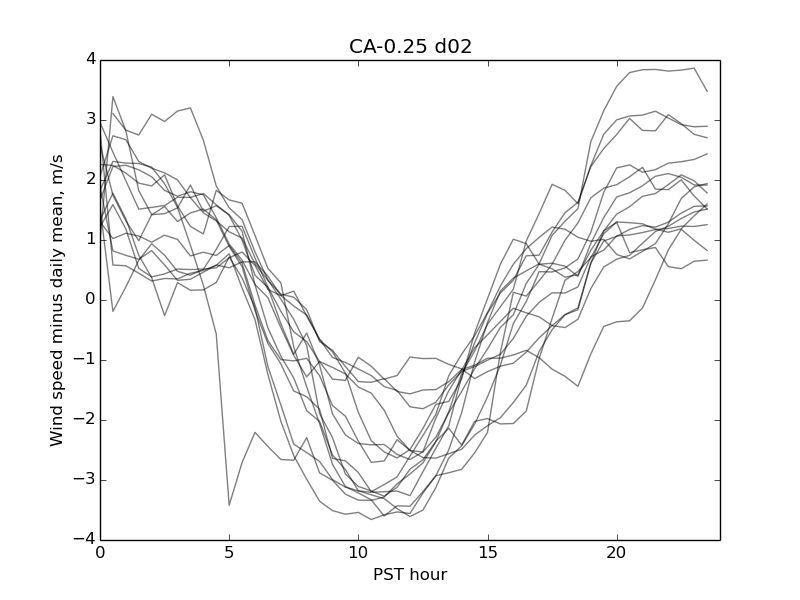
\includegraphics[width=1\textwidth]{ch3-wind/img/solano_controlwind_minusmean_CA0pt25_d02_level0.png}
\caption{}
\end{subfigure}
\begin{subfigure}{0.5\textwidth}
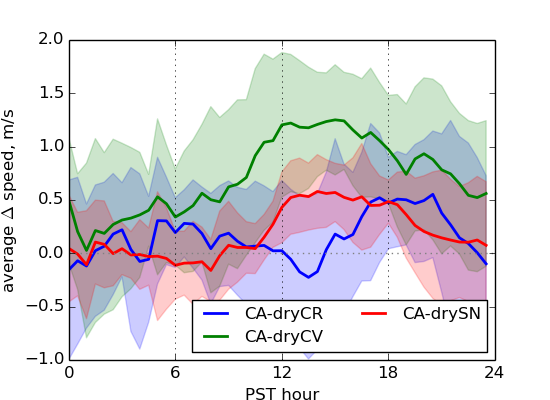
\includegraphics[width=1\textwidth]{ch3-wind/img/solano_diurnalwind_dry_regions_d02_level0.png}
\caption{}
\end{subfigure}
\caption{(a) Overlaid diurnal cycles of wind speed magnitude minus daily mean wind speed, at 60 m AGL for the d02 grid point nearest the Solano wind farm, for the CA-0.25 control case.  (b) Diurnally averaged differences in wind speed, at 60 m AGL for the d02 grid point nearest the Solano wind farm, for the wet background/dry perturbation cases.  Shading represents one standard deviation.}
\label{fig:windSol_DiffDiurnalDryRg}
\end{figure}

\begin{figure}[here]
\begin{subfigure}{0.5\textwidth}
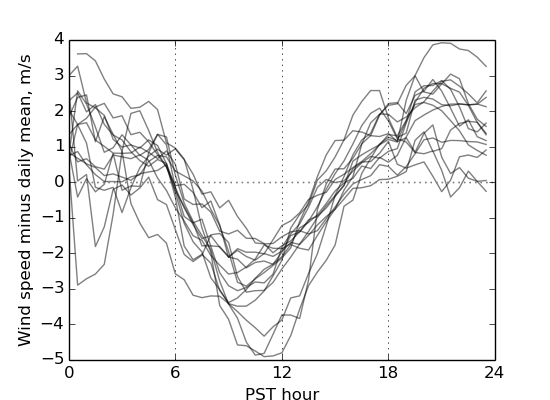
\includegraphics[width=1\textwidth]{ch3-wind/img/solano_controlwind_minusmean_CA0pt1_d02_level0.png}
\caption{}
\end{subfigure}
\begin{subfigure}{0.5\textwidth}
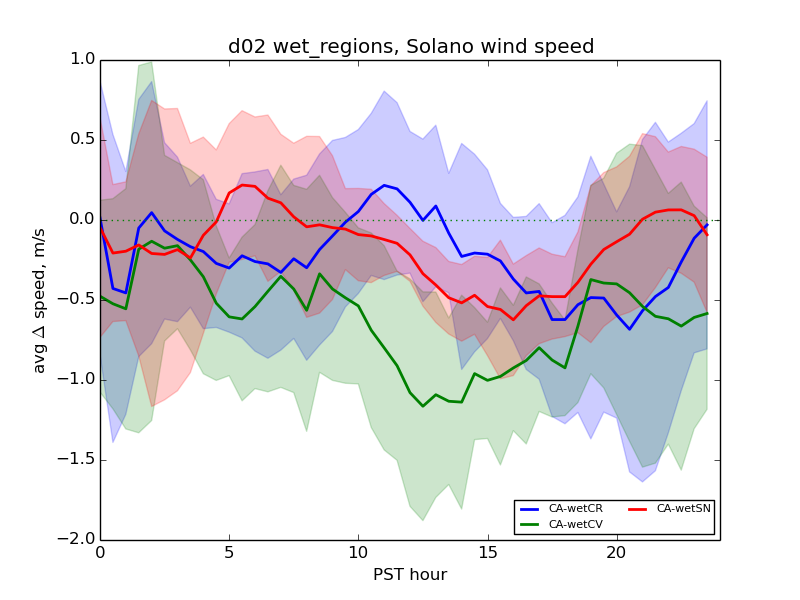
\includegraphics[width=1\textwidth]{ch3-wind/img/solano_diurnalwind_wet_regions_d02_level0.png}
\caption{}
\end{subfigure}
\caption{(a) Overlaid diurnal cycles of wind speed magnitude minus daily mean wind speed, at 60 m AGL for the d02 grid point nearest the Solano wind farm, for the CA-0.1 control case.  (b) Diurnally averaged differences in wind speed, at 60 m AGL for the d02 grid point nearest the Solano wind farm, for the dry background/wet perturbation cases.  Shading represents one standard deviation.}
\label{fig:windSol_DiffDiurnalWetRg}
\end{figure}

\begin{figure}[here]
\begin{subfigure}{0.49\textwidth}
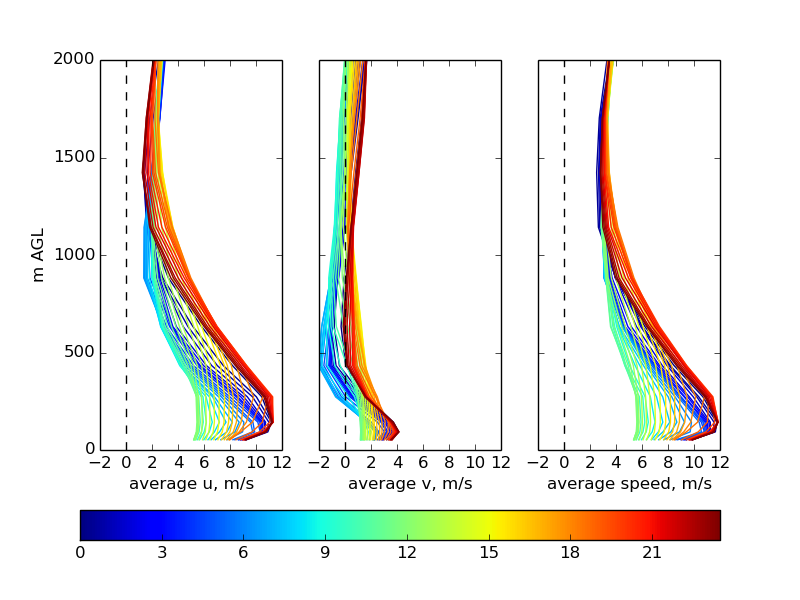
\includegraphics[width=\textwidth]{ch3-wind/img/windprof_hr_avg_CA0pt25.png}
\caption{}
\end{subfigure}
\begin{subfigure}{0.49\textwidth}
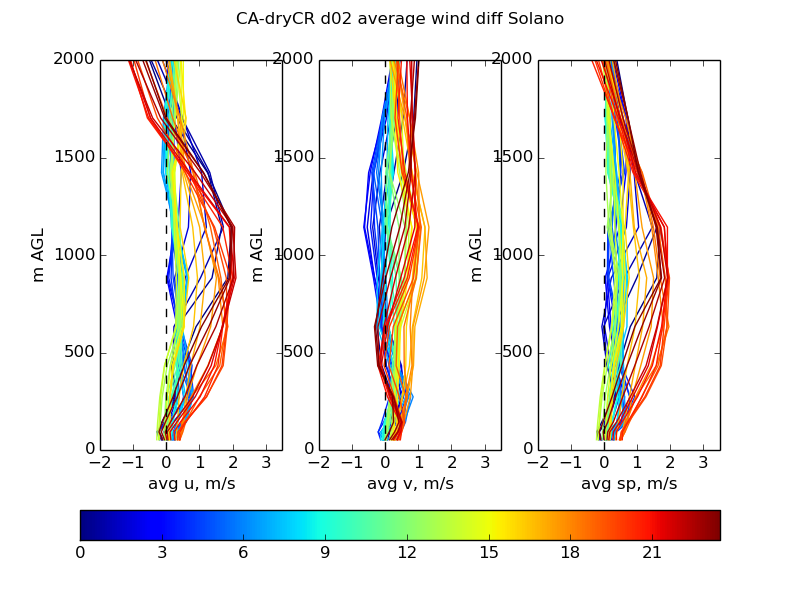
\includegraphics[width=\textwidth]{ch3-wind/img/windprof_diff_hr_avg_dryCR.png}
\caption{}
\end{subfigure}
\begin{subfigure}{0.49\textwidth}
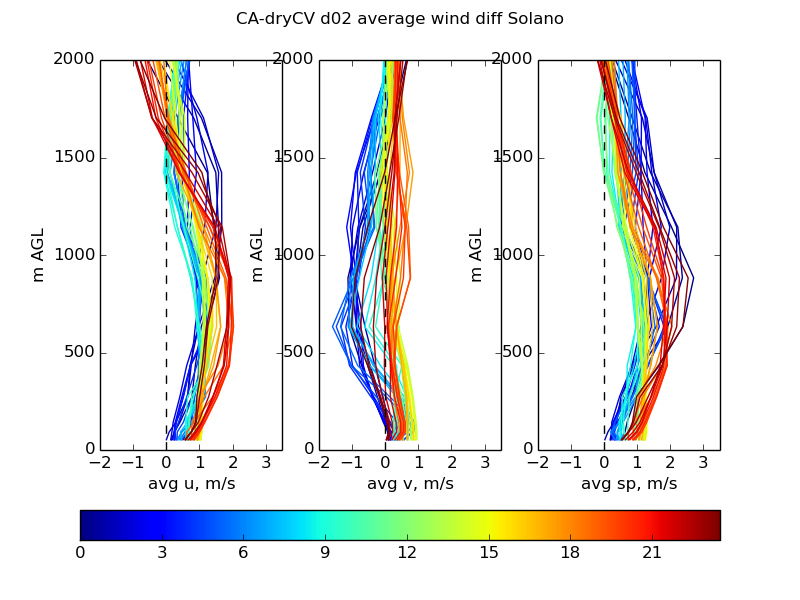
\includegraphics[width=\textwidth]{ch3-wind/img/windprof_diff_hr_avg_dryCV.png}
\caption{}
\end{subfigure}
\begin{subfigure}{0.49\textwidth}
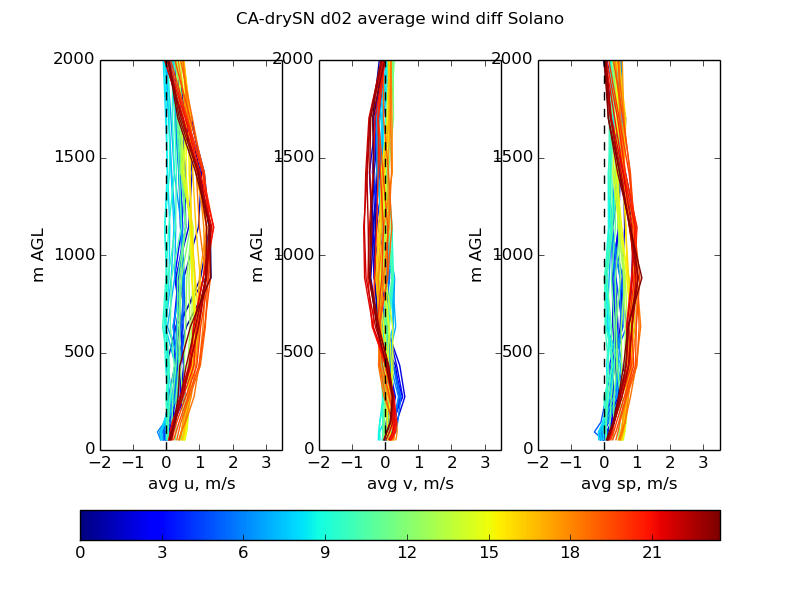
\includegraphics[width=\textwidth]{ch3-wind/img/windprof_diff_hr_avg_drySN.png}
\caption{}
\end{subfigure}
\caption{Vertical profiles of $u$, $v$, and $|u|$, averaged by time of day over the whole simulation (colorbar indicates hour of day in local time), for (a) CA-0.25 control run, and averaged differences from control run for the dry regional test cases: (b) dryCR, (c) dryCV, (d) drySN.}
\label{fig:windSol_VertProfileDryRg}
\end{figure}

\subsubsection{Regional sensitivity}

The Solano wind changes occur in the context of larger regional wind and pressure changes (Figure \ref{fig:windSol_WindMapsRg}).  In all dry regional tests, the pressure gradient and wind increase throughout the Central Valley, most strongly in the afternoon (second and third rows in Figure \ref{fig:windSol_WindMapsRg}).  In the dry Coast Range test (Figure \ref{fig:windSol_WindMapsRg} (e)-(h)), the pressure in the northern Central Valley decreases and wind in the northern Central Valley strengthens as cyclonic flow develops around the northern Coast Range.  In the dry Central Valley test (Figure \ref{fig:windSol_WindMapsRg} (i)-(l)), the pressure gradient from the San Francisco Bay to the Central Valley increases dramatically at 14:00, and these increases persist at 18:00 and to a lesser degree at 00:00. However, at 18:00, the zone of steepest pressure change has been pushed further eastward, and the strongest wind increases track this band of largest pressure gradient.  The pattern of wind increases at 00:00 is disorganized, and wind speeds decrease in the southern Central Valley at 06:00.  In the dry Sierra Nevada case (Figure \ref{fig:windSol_WindMapsRg} (m)-(p)), the pressure gradient strengthens moderately at 14:00 and 18:00, but pressure changes are minimal by 00:00 and 06:00.  Wind speeds increase through the Solano pass and the middle Central Valley in the afternoon (14:00 and 18:00), and by 18:00, the bands of largest wind increases have moved outward along Central Valley, again following zones of greatest pressure gradient increase.  Wind changes at night (00:00 and 06:00) are small and disorganized.

%The Solano wind in the regional test cases differs from the control case by as much as 2 m/s, and the largest changes occur when Central Valley soil moisture is perturbed (dryCV and wetCV).  

For all regional test cases, drier soils on a wet background increase Solano winds in the afternoon and evening relative to the all-wet control (Figure \ref{fig:windSol_DiffDiurnalDryRg}(b)); this increase is largest in the dryCV case.  The increases in both the dryCV and drySN cases are greatest between 11:00 and 18:00 (0.8-1.8 m/s for dryCV and 0.25-0.8 m/s for drySN), while the increase in the dryCR case happens later, between 17:00 and 22:00 (0.25-1 m/s).  Importantly, increases in the afternoon cause the daily wind speed ramp-up to shift earlier, because the increases occur at the same time as the control ramp-up (Figure \ref{fig:windSol_DiffDiurnalDryRg}(a)).  Because there are no corresponding decreases at the hour of ramp-down, this means that the duration of the high-wind period also increases.  Also, drier soils (especially in the Central Valley) increase the minimum wind (08:00 to 13:00) on many individual days (Figure \ref{fig:windSol_TseriesDryRg}), but the average increases in the minimum wind are not more than one standard deviation greater than zero in the two-week average diurnal cycle (Figure \ref{fig:windSol_DiffDiurnalDryRg}(b)).

Wetter soils on a dry background cause winds to decrease relative to the all-dry control case, and the magnitudes of the decreases are similar to the magnitudes of the increases in the dry regional tests (Figure \ref{fig:windSol_DiffDiurnalWetRg}(b)).  Again, the decrease is largest in when Central Valley soil moisture is perturbed.  Both the wetCV and wetSN cases have wind decreases during 10:00-18:00 that are more than one standard deviation from zero (0.5-1.8 m/s for wetCV and 0.25-0.8 m/s for wetSN); for the wetCR case, there are no times of day with wind changes more than one standard deviation from zero, although there are weak decreases in the late afternoon and evening.

In summary, the Central Valley soil moisture influences the Solano turbine-level winds more strongly than does the Coast Range or Sierra Nevada soil moisture.  Drier soils in all regions, but especially in the Central Valley, increase Solano wind speeds during ramp-up and peak hours (afternoon and evening); drier soils in the Central Valley, especially, shift the daily wind ramp-up earlier.  Conversely, wetter Central Valley soils cause Solano winds to decrease during ramp-up and peak times.

\subsubsection{Scaling of wind changes with Central Valley soil moisture}

\begin{figure}[here]
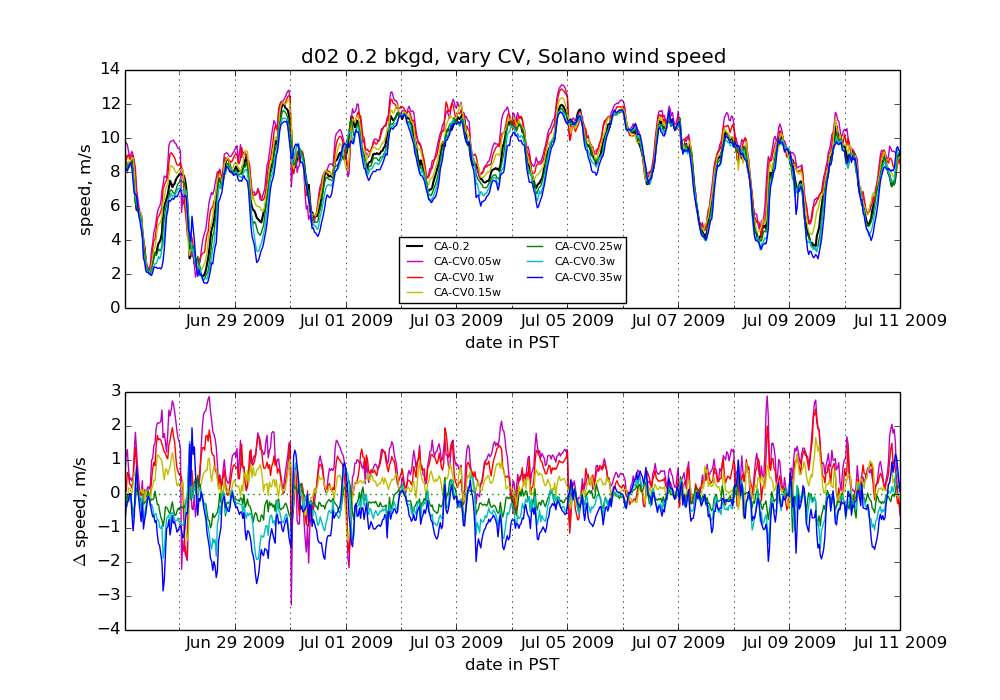
\includegraphics[width=1\textwidth]{ch3-wind/img/solano_wind_CV0pt2_d02_level0.png}
\caption{Time series of wind speed magnitude at 60 m AGL for the d02 grid point nearest the Solano wind farm, for a range of Central Valley soil moisture values, with soil moisture = 0.2 in the Coast Range and Sierra Nevada.  (a) Wind speed time series, (b) time series of differences between test cases and control (CA-0.2).  The model spin-up period is excluded.}
\label{fig:windSol_TseriesWindCV}
\end{figure}

\begin{figure}[here]
\begin{subfigure}{0.6\textwidth}
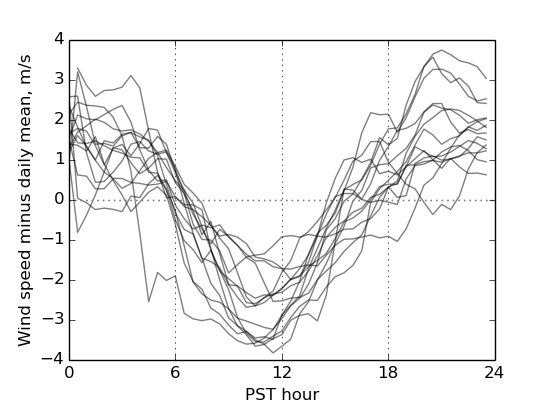
\includegraphics[width=1\textwidth]{ch3-wind/img/solano_controlwind_minusmean_CA0pt2_d02_level0.png}
\caption{}
\end{subfigure}
\begin{subfigure}{0.6\textwidth}
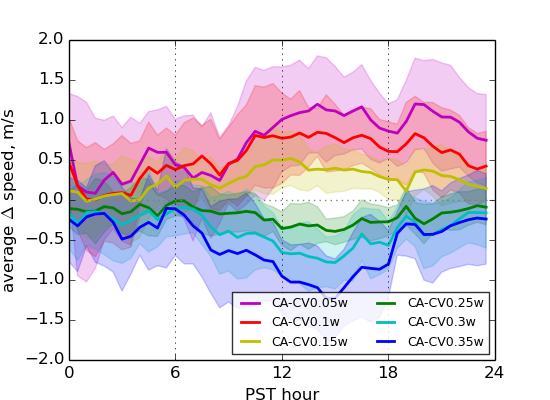
\includegraphics[width=1\textwidth]{ch3-wind/img/solano_diurnalwind_CV_0pt2_d02_level0.png}
\caption{}
\end{subfigure}
\caption{(a) Overlaid diurnal cycles of wind speed magnitude minus daily mean wind speed, at 60 m AGL for the d02 grid point nearest the Solano wind farm, for the CA-0.2 control case.  (b) Diurnally averaged differences in wind speed, at 60 m AGL for the d02 grid point nearest the Solano wind farm, for a range of Central Valley soil moisture values.  Shading represents one standard deviation.}
\label{fig:windSol_DiffDiurnalCV0pt2}
\end{figure}

\begin{figure}[here]
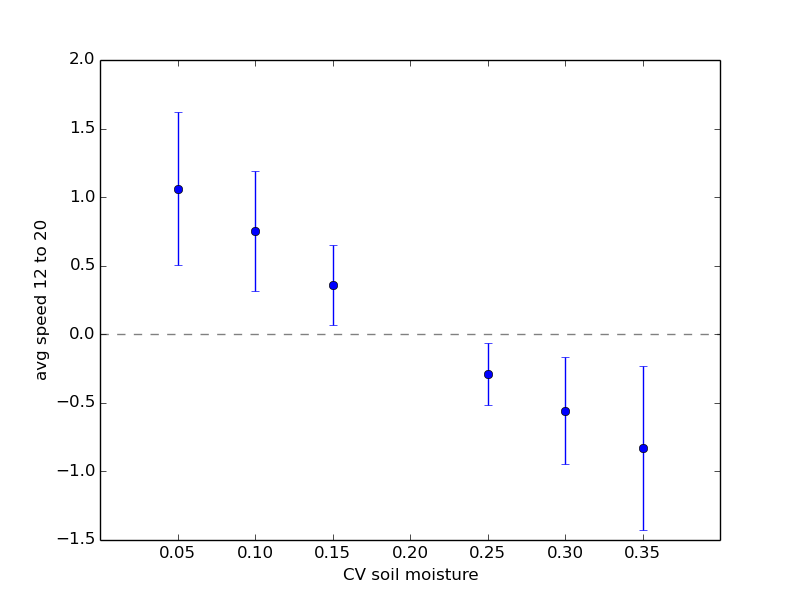
\includegraphics[width=1\textwidth]{ch3-wind/img/shifts_CVsmois_12-20_d02.png}
\caption{Average changes in wind speed between hours 12:00 and 20:00, for different values of CV soil moisture with CR and SN soil moisture set to 0.2 m$^3$/m$^3$.  Changes are relative to the CA-0.2 control case.  Error bars represent one standard deviation.}
\label{fig:windSol_ShiftsMaxCV}
\end{figure}

Drier Central Valley soils increase Solano winds, while wetter Central Valley soils decrease Solano winds, relative to the moderately wet control of soil moisture = 0.2 (Figure \ref{fig:windSol_TseriesWindCV}.)  These changes can be up to 3 m/s, and they occur most consistently in the hours of 12:00 to 22:00 (Figure \ref{fig:windSol_DiffDiurnalCV0pt2}(b)), when they are 0.8-1.7 m/s on average in the driest Central Valley case (CV0.05).  The average changes during hours 12:00 to 22:00 scale slightly nonlinearly with CV soil moisture (Figure \ref{fig:windSol_ShiftsMaxCV}), with larger increases in wind per unit soil moisture decrease when the Central Valley soil is drier than 0.2 m$^3$/m$^3$.  The greater sensitivity of wind to soil moisture when soils are drier may be due to a greater sensitivity of surface heating to soil moisture when soils are drier, because of rapid declines in soil hydraulic conductivity and plant stomatal conductance in the moderate-to-dry soil moisture range (\textbf{cite something � Bonan? Sap flow paper? Transitional soil moisture regime paper of some kind?}).

\clearpage

\subsection{Physical mechanism}
\label{subsec:PhysMech}

Next we investigate the physical mechanism by which changes in soil moisture, especially in the Central Valley, influence near-surface winds at Solano.  

The strong diurnal component of the Solano wind (Figures \ref{fig:windSol_TseriesDryRg} and \ref{fig:windSol_TseriesWetRg}) and the wind speed peak at low levels (Figure \ref{fig:windSol_VertProfileDryRg}) suggest significant forcing by land surface heating (consistent with Zhong \textit{et al.} [2004] and Mansbach [2010]).  In order to explore the influence of land surface forcing on terms in the momentum budget, we model the topographically channeled wind at Solano as simple one-dimensional flow through the pass governed by a one-dimensional momentum equation,

\begin{equation}
\frac{\partial u}{\partial t} = -u\frac{\partial u}{\partial x} -\frac{1}{\rho} \frac{\partial p}{\partial x} - F\left(\frac{\partial u}{\partial z}, N\right),
\label{eqn:windSol_momentum}
\end{equation}
neglecting the Coriolis term because of the topographic constraint on wind direction.  The first term on the right hand side is the advection of momentum, the second term is the pressure gradient force, and the third term is frictional dissipation as an unspecified function of vertical wind shear and stability (quantified by $N$, the Brunt-V\"ais\"al\"a frequency).  We are interested in the importance of each of these terms through the diurnal cycle and in the influence of soil moisture changes on each of these terms.

\subsubsection{Driving pressure gradient}

\begin{figure}[here]
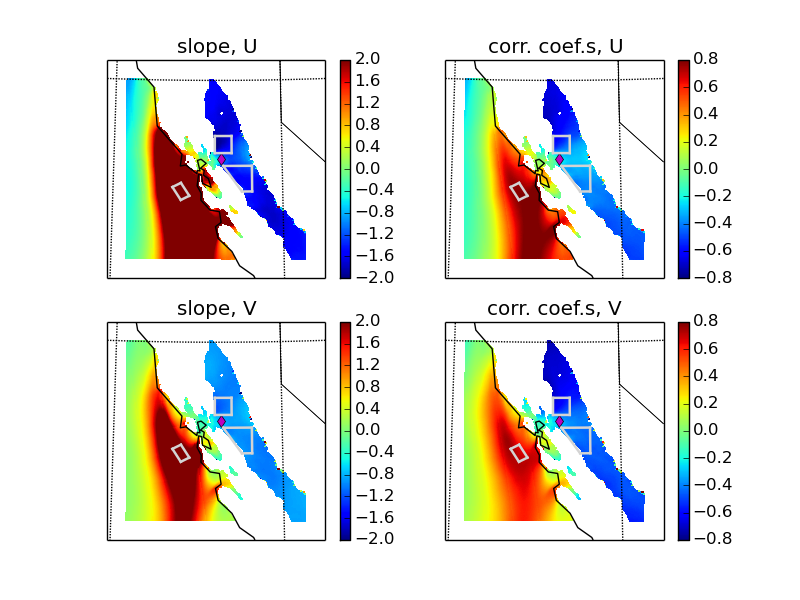
\includegraphics[width=1\textwidth]{ch3-wind/img/corr_wind_panom_lev110_lag12_CA0pt25.png}
\caption{CA-0.25 case: Solano 60 m AGL (110 m ASL) wind linearly regressed against horizontal pressure anomaly at 110 m ASL, with wind lagging pressure by 6 hours.  Top row: $u$-component of wind; bottom row: $v$-component of wind.  Left column: linear regression slope; right column: correlation coefficient.  Gray boxes outline areas used to calculate pressure gradients; ocean box is ``OCN", northern box in the Central valley is ``NCV", and southern box in Central Valley is ``SCV".}
\label{fig:windSol_CorrMap0pt25}
\end{figure}

\begin{figure}[here]
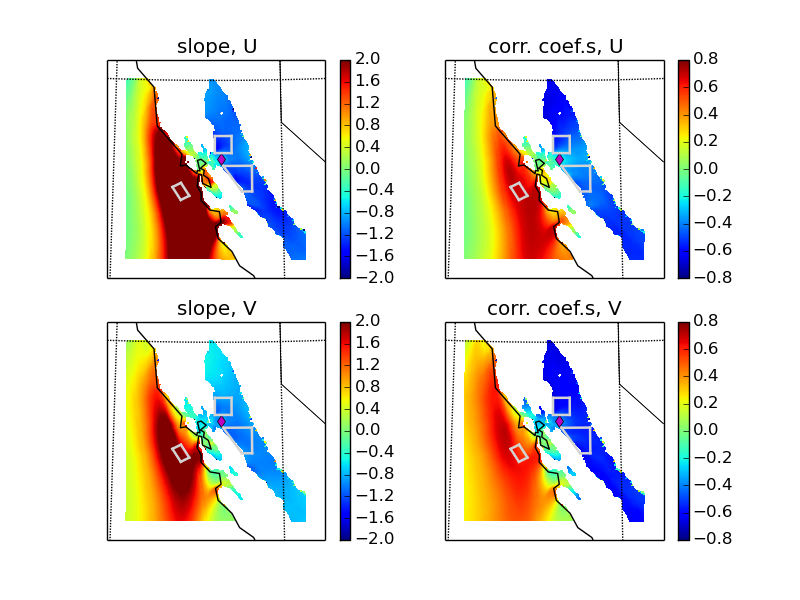
\includegraphics[width=1\textwidth]{ch3-wind/img/corr_wind_panom_lev110_lag12_CA0pt1.png}
\caption{CA-0.1 case: Solano 60 m AGL (110 m ASL) wind linearly regressed against horizontal pressure anomaly at 110 m ASL, with wind lagging pressure by 6 hours.  Top row: $u$-component of wind; bottom row: $v$-component of wind.  Left column: linear regression slope; right column: correlation coefficient.}
\label{fig:windSol_CorrMap0pt1}
\end{figure}

In order to identify the pressure gradient most relevant to Solano winds, we linearly regress the horizontal pressure anomaly, calculated at each output time step, against Solano turbine-level wind.  The regression is repeated for pressure at a range of heights and for a range of lag times, with wind lagging pressure.  The regression slopes and correlation coefficients for the control cases (CA-0.25, Figure \ref{fig:windSol_CorrMap0pt25}, and CA-0.1, Figure \ref{fig:windSol_CorrMap0pt1}) show a consistent pattern of positive slopes and correlation coefficients over the ocean near the central coast (meaning higher pressure in those regions corresponds to faster wind), and negative slopes and correlation coefficients throughout the Central Valley, especially just north and south of the Solano pass (meaning lower pressure in those regions corresponds to faster wind).

\begin{figure}[here]
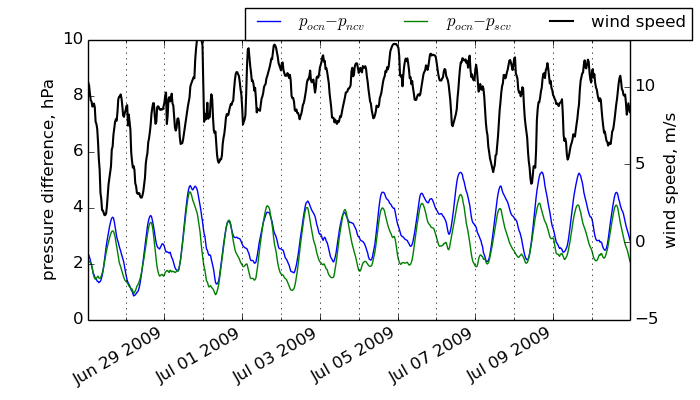
\includegraphics[width=1\textwidth]{ch3-wind/img/pgrad_wind_CA0pt1_level110.png}
\caption{CA-0.1 control case: Solano 60 m AGL (110 m ASL) wind (black) and average pressure difference OCN box minus NCV box (blue) and OCN box minus SCV box (green) at 110 m ASL.  The sign of the pressure difference is chosen to correspond with the $\frac{-1}{\rho} \frac{\partial p}{\partial x}$ term in the momentum budget.}
\label{fig:windSol_PgradWind}
\end{figure}

\begin{figure}[here]
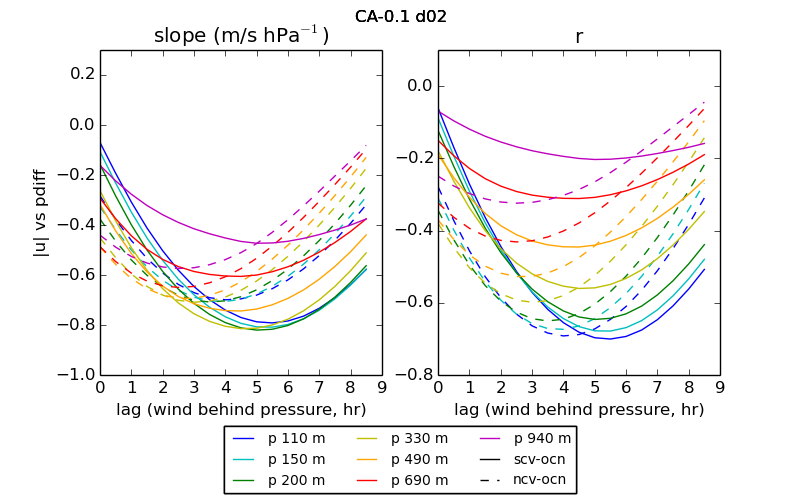
\includegraphics[width=1\textwidth]{ch3-wind/img/lag_corr_pdiff_combo_ncv_scv_d02_CA0pt1.png}
\caption{CA-0.1 control case: lagged linear regression of Solano 60 m AGL (110 m ASL) wind against average pressure difference NCV box minus OCN box (dashed) and SCV box minus OCN box (solid).  Correlations are only shown for speed, because u and v velocity component results are very similar.}
\label{fig:windSol_LagCorrCtrl}
\end{figure}

Based on this finding, we choose three boxes, shown in gray in Figures \ref{fig:windSol_CorrMap0pt25} to \ref{fig:windSol_CorrMap0pt1}, to represent the pressure gradient driving Solano winds.  The lag of wind speed behind pressure gradient is evident in the time series of Solano wind and pressure difference between the boxes (Figure \ref{fig:windSol_PgradWind}).  Not only does the pressure difference peak 5-6 hours before the Solano wind speed, but the peak pressure difference rapidly dissipates (beginning to decline after 1-2 hours), while the peak wind speed persists for 6-8 hours.  Using the pressure difference between the three boxes, we confirm that the peak sensitivity (as measured by the regression slope) and correlation occur with pressure at 110 m ASL (although the metrics are high at all levels below $\sim$300 m) with a lag of $\sim$4-5 hr for NCV-OCN pressure and $\sim$5-6.5 hr for SCV-OCN pressure (Figure \ref{fig:windSol_LagCorrCtrl}).

\begin{figure}[here]
\begin{subfigure}{0.6\textwidth}
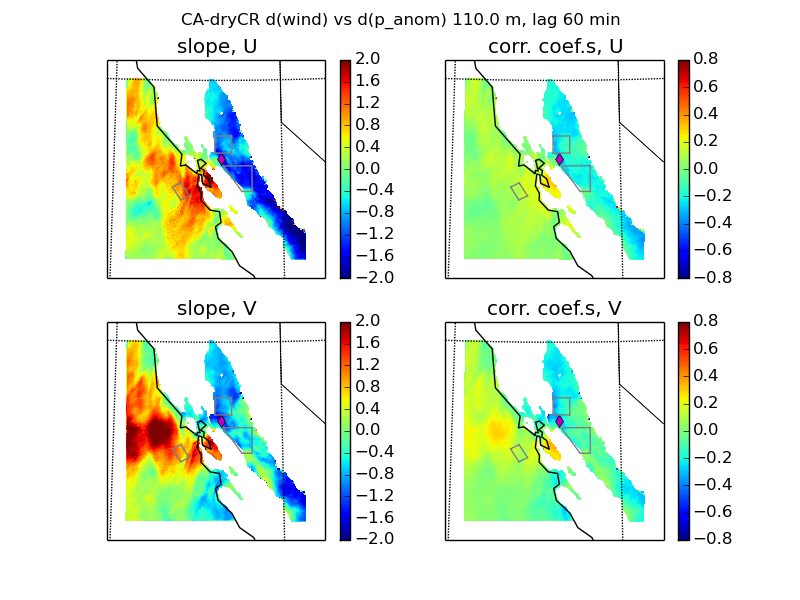
\includegraphics[width=\textwidth]{ch3-wind/img/corr_dwind_dpanom_lev110_lag2_dryCR.png}
\caption{}
\end{subfigure}
\begin{subfigure}{0.6\textwidth}
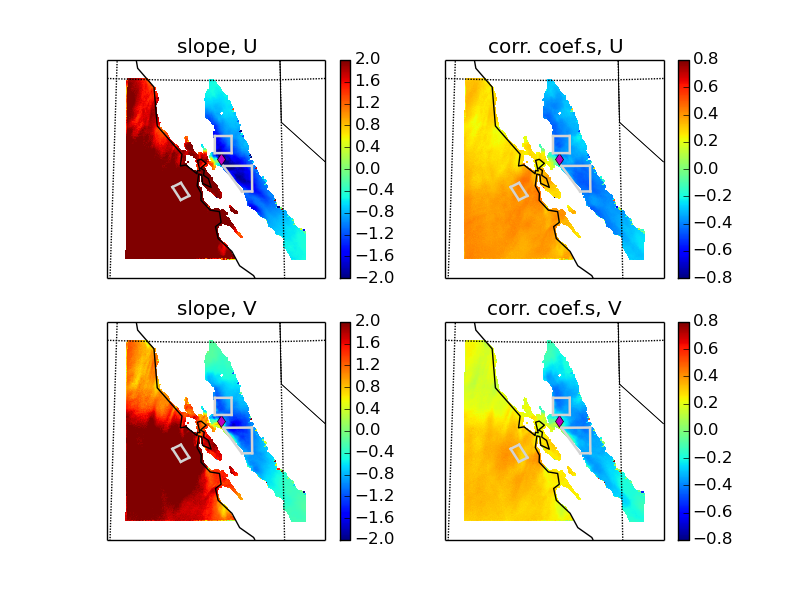
\includegraphics[width=\textwidth]{ch3-wind/img/corr_dwind_dpanom_lev110_lag2_dryCV.png}
\caption{}
\end{subfigure}
\begin{subfigure}{0.6\textwidth}
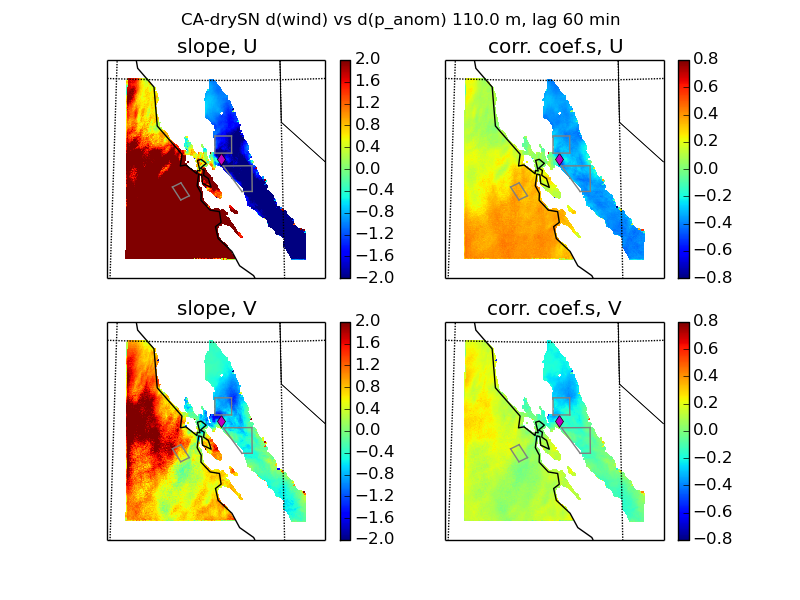
\includegraphics[width=\textwidth]{ch3-wind/img/corr_dwind_dpanom_lev110_lag2_drySN.png}
\caption{}
\end{subfigure}
\caption{Correlation between Solano wind changes at 60 m AGL and horizontal pressure anomaly of change in 110 m ASL pressure, with a lag of 60 min, for the dry regional test cases minus control: (a) dryCR, (b) dryCV, (c) drySN.  The order of panels is as in Figure \ref{fig:windSol_CorrMap0pt25}.}
\label{fig:windSol_CorrMapDryRg}
\end{figure}

\begin{figure}[here]
\begin{subfigure}{0.6\textwidth}
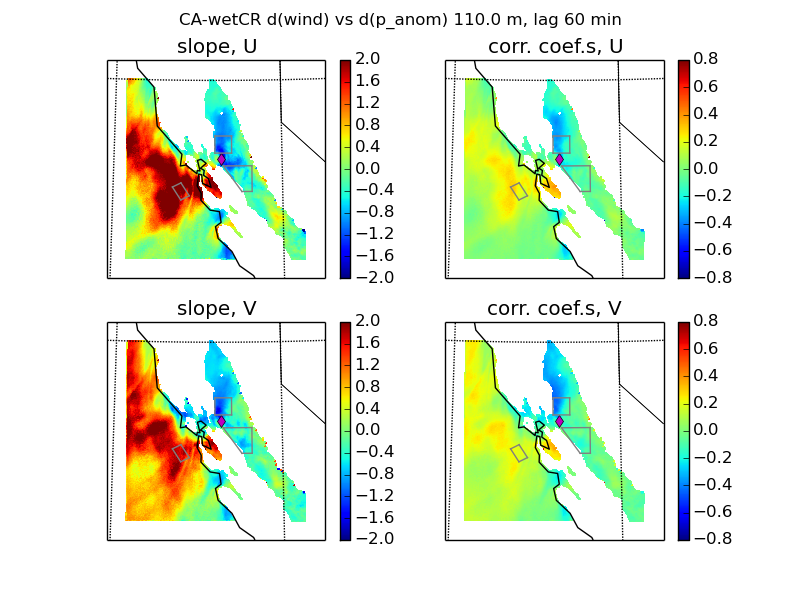
\includegraphics[width=\textwidth]{ch3-wind/img/corr_dwind_dpanom_lev110_lag2_wetCR.png}
\caption{}
\end{subfigure}
\begin{subfigure}{0.6\textwidth}
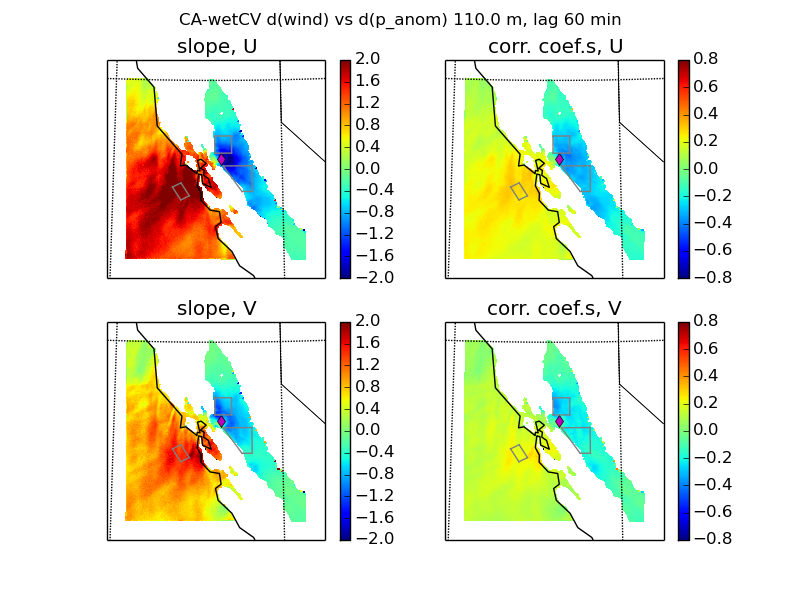
\includegraphics[width=\textwidth]{ch3-wind/img/corr_dwind_dpanom_lev110_lag2_wetCV.png}
\caption{}
\end{subfigure}
\begin{subfigure}{0.6\textwidth}
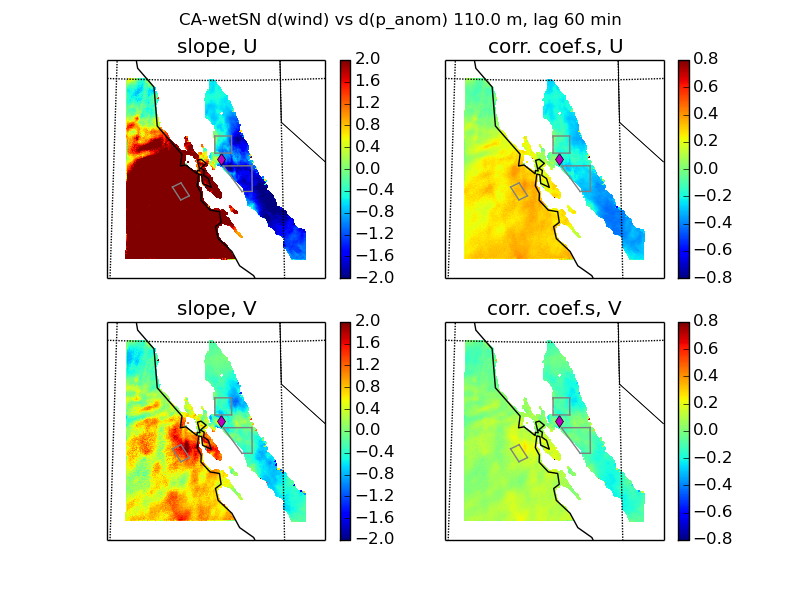
\includegraphics[width=\textwidth]{ch3-wind/img/corr_dwind_dpanom_lev110_lag2_wetSN.png}
\caption{}
\end{subfigure}
\caption{Correlation between Solano wind changes at 60 m AGL and horizontal pressure anomaly of change in 110 m ASL pressure, with a lag of 60 min, for the wet regional test cases minus control: (a) wetCR, (b) wetCV, (c) wetSN.  The order of panels is as in Figure \ref{fig:windSol_CorrMap0pt25}.}
\label{fig:windSol_CorrMapWetRg}
\end{figure}

\begin{figure}[here]
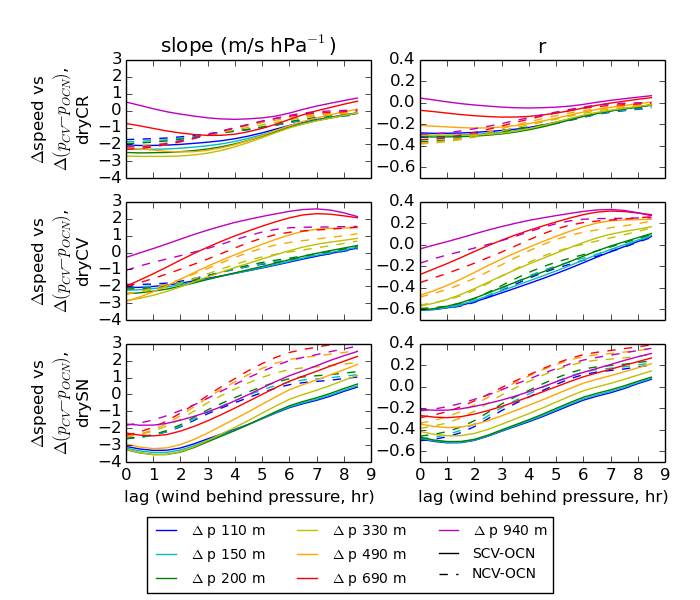
\includegraphics[width=1\textwidth]{ch3-wind/img/lag_corr_dpdiff_combo_ncv_scv_d02_testminusctrl.png}
\caption{Dry regional perturbation cases: lagged linear regression of test-minus-control Solano 60 m AGL (110 m ASL) wind against test-minus-control average pressure difference NCV box minus OCN box (dashed) and SCV box minus OCN box (solid).  Top row: dryCR; middle row: dryCV; bottom row: drySN.}
\label{fig:windSol_LagCorrTest}
\end{figure}

Repeating the regression analysis using test-minus-control changes in pressure and Solano wind, a similar spatial pattern of sensitivity emerges (positive correlation between Solano wind changes and pressure changes in the central coastal ocean, and negative correlation between Solano wind changes and pressure changes in the Central Valley), albeit with weaker correlation (Figures \ref{fig:windSol_CorrMapDryRg} and \ref{fig:windSol_CorrMapWetRg}).  Again, the changes in wind speed correlate maximally with the changes in pressure at the lowest altitudes ($\le$ 200 m, Figure \ref{fig:windSol_LagCorrTest}).  In contrast to the control cases which have a 5-6 hour lag, the test-minus-control changes correlate maximally at a lag of $\le$ 1 hour (Figure \ref{fig:windSol_LagCorrTest}).

\subsubsection{Temperature controls on pressure}

\begin{figure}[here]
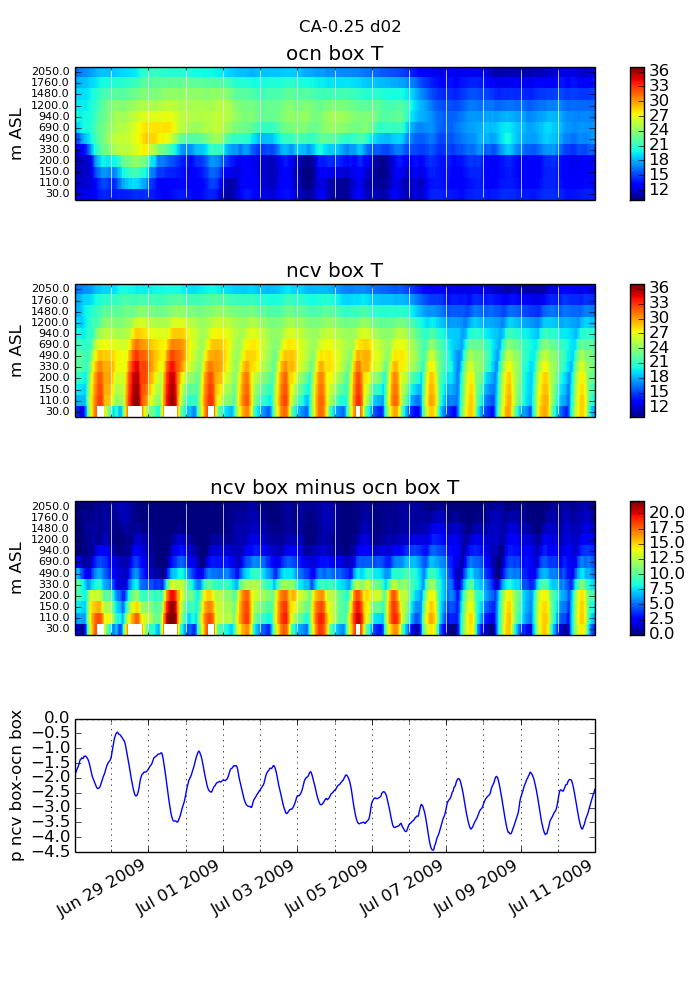
\includegraphics[width=0.9\textwidth]{ch3-wind/img/timeheight_T_pdiff_ocnbox_ncvbox_0pt25.png}
\caption{CA-0.25 control case: Temporal evolution of the vertical profile of temperature for the OCN box (top panel), the NCV box (second panel), NCV minus OCN (third panel); and time series of the NCV minus OCN pressure at 110 m ASL (bottom panel).  White areas indicate times when the lowest $\sigma$ model level was higher than 30 m ASL for the NCV box.}
\label{fig:windSol_TimeHeightCtrl}
\end{figure}

The diurnal variations in low-level pressure correspond to diurnal variations in boundary layer temperature, because pressure is the vertical integral of the weight of the air column above a point, and changes in temperature change the density and thus the weight of the air column.  Diurnal temperature variations are larger in the Central Valley than over the ocean (Figure \ref{fig:windSol_TimeHeightCtrl}).  In the NCV box, the temperature near the surface (\textless 100 m ASL) declines quickly after sunset, but the temperature aloft in the boundary layer (particularly 300-700 m) remains elevated until at least midnight (Figure \ref{fig:windSol_TimeHeightCtrl}, panel 2).  Both the NCV temperature and the NCV-OCN temperature difference peak around 17:00.  The temperature difference at low levels (\textless 110 m) drops after sunset and approaches zero in the early morning some days, but the temperature difference remains positive at 110-490 m on most days, with NCV warmer than OCN by up to 12 deg C even in the early morning.  The near-surface cooling in the Central Valley is due to a combination of radiative cooling of the land surface and advection of cooler marine air by the low-level wind maximum.  The pressure difference is most negative (strongest gradient) at the same time as the maximum temperature difference, around 17:00, and is smallest in magnitude (weakest gradient) just before sunrise, around 06:00, when the NCV boundary layer is coolest.  

\begin{figure}[here]
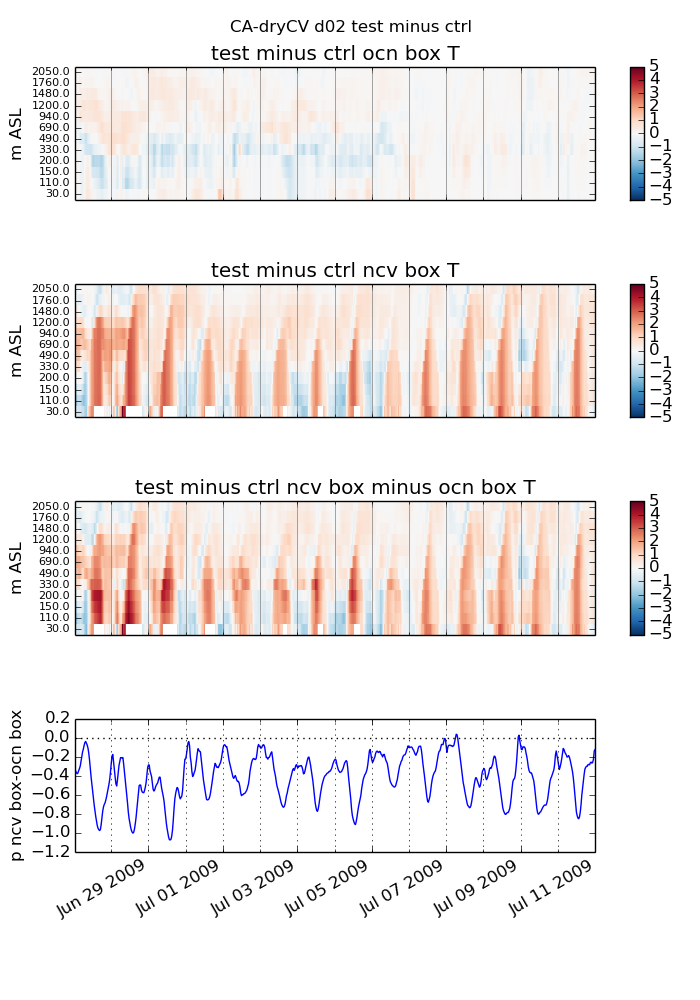
\includegraphics[width=0.9\textwidth]{ch3-wind/img/timeheight_T_pdiff_ocnbox_ncvbox_diff_dryCV.png}
\caption{dryCV case: Temporal evolution of the vertical profile of test-minus-control temperature changes for the OCN box (top panel), the NCV box (second panel), NCV minus OCN (third panel); and time series of test-minus-control changes in the NCV minus OCN pressure at 110 m ASL (bottom panel).  White areas indicate times when the lowest $\sigma$ model level was higher than 30 m ASL for the NCV box.}
\label{fig:windSol_TimeHeightDryCV}
\end{figure}

Changes in soil moisture affect the pressure gradient by changing surface heat fluxes and thus air temperature.  Temperature changes in the lower 1000 m of the NCV box are much larger in the dryCV case than in the dryCR or drySN cases; as such, only the dryCV case is shown (Figure \ref{fig:windSol_TimeHeightDryCV}).  We note that in the dryCR and drySN cases, temperature and pressure changes are much smaller (+/- 1 degree C and -0.4 hPa), and the pressure gradient strengthens in the late afternoon, largely corresponding to warming at boundary layer levels above the surface (150 m to 1200 m).

In the dryCV case, the NCV experiences strong low-level heating beginning in the morning, increasing in altitude as the boundary layer grows; temperature increases during day are well-mixed in the boundary layer.  There is mild cooling over the OCN box at 200-330 m in the first week of the simulation.  The strongest increase in temperature difference (warming of NCV relative to OCN) occurs late morning to late afternoon, at all levels below 690 m.  At night, there is a small decrease in the low-level (\textless 330 m) temperature difference.  The corresponding strengthening of the pressure difference is also greatest from late morning to late afternoon.  The mild strengthening of the pressure gradient on some nights (e.g. early morning of June 28, June 29, July 3, July 8) appears related to longer nocturnal persistence of warming at NCV relative to OCN in the residual boundary layer (150 m - 690 m, although the elevation of warming differs among individual days).

\subsubsection{Momentum budget timing and changes}

\begin{figure}[here]
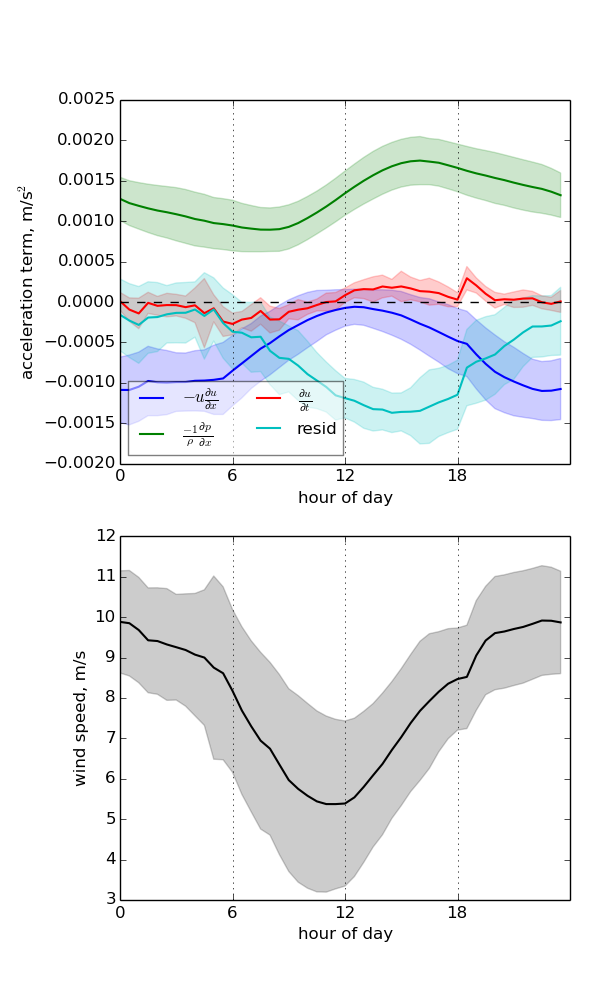
\includegraphics[width=0.9\textwidth]{ch3-wind/img/momentum_terms_diurnal_0pt25.png}
\caption{CA-0.25 control case: Diurnal average of terms of the momentum balance.  Pressure gradient is calculated between the NCV and OCN boxes, and using density calculated at Solano 60 m AGL.  Advection is calculated as $u_{solano}\frac{\partial u}{\partial x}$ with $\frac{\partial u}{\partial x}$ estimated with the gradient in wind between Solano and San Pablo Bay (the northern part of the San Francisco Bay).  $\frac{\partial u}{\partial t}$ is calculated using Solano 60 m AGL wind speed.  Friction (cyan) is calculated as the residual of the other three terms, following Equation \ref{eqn:windSol_momentum}.  Shading represents one standard deviation.}
\label{fig:windSol_MomTermsDiurn}
\end{figure}

The momentum advection, pressure gradient, and $u$ time tendency terms in Equation \ref{eqn:windSol_momentum} are estimated from model output for the CA-0.25 control (Figure \ref{fig:windSol_MomTermsDiurn}).  Using these three model-derived terms, we calculate the friction term as the residual (Figure \ref{fig:windSol_MomTermsDiurn}, cyan line).  The friction term has to vary diurnally in order to reproduce the observed wind diurnal cycle.  The time tendency ($\frac{\partial u}{\partial t}$) term is much smaller than pressure gradient term, even in afternoon when the pressure gradient is largest and advection is small.  If friction were not also large at this time, the wind would accelerate much faster.  Conversely, high wind speeds persist even after the pressure gradient declines between 22:00 and 04:00 and despite the strong advection of lower momentum air.  If friction during the night remained at its high afternoon values, the winds would decelerate at night.  The decline in the friction term at night is necessary in order to explain the observed high winds at night.  [\textbf{cite LLJ paper of some sort - not the first time this is being said.}]  Moreover, this residual has the expected diurnal shape of friction, with high values in the daytime when convective turbulence creates a uniform boundary layer and high momentum flux to the ground, and low values at night when the residual upper boundary layer decouples from the shallow stable nocturnal boundary layer and is buffered from friction with the surface.
% Indeed, the diurnal course of modeled $u*$ at Solano has the same timing as the $F(\frac{\partial u}{\partial z}, N)$ term calculated from the residual (ustar figure).

\begin{figure}[here]
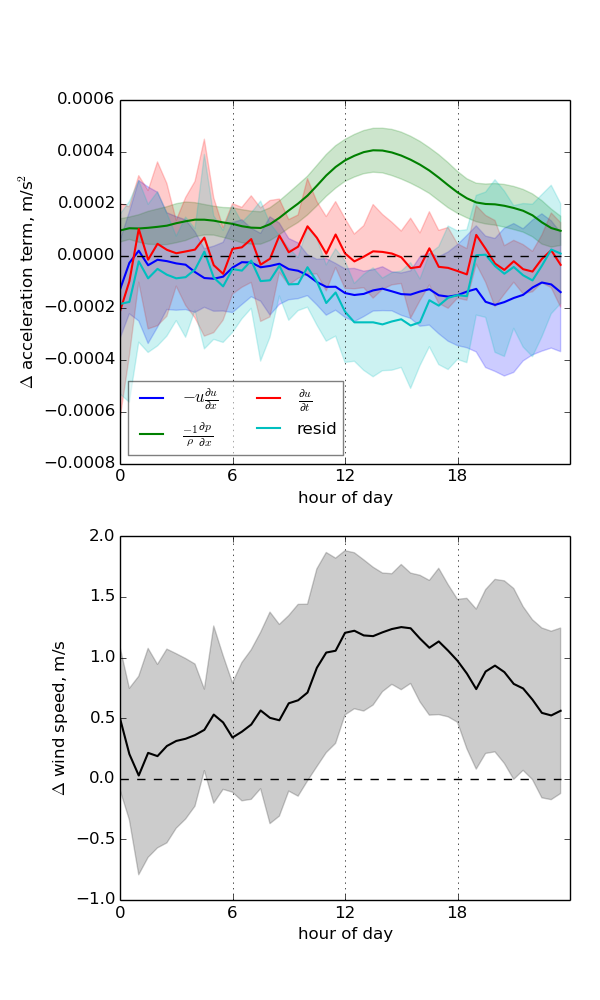
\includegraphics[width=0.9\textwidth]{ch3-wind/img/momentum_terms_diurnal_diff_dryCV.png}
\caption{dryCV case: Diurnal average of test-minus-control change in terms of the momentum balance, calculated as in Figure \ref{fig:windSol_MomTermsDiurn}.  Shading represents one standard deviation.}
\label{fig:windSol_MomTermsDiurnDiff}
\end{figure}

In the dryCV case, the pressure gradient term increases at all hours but especially between 10:00 and 18:00 (Figure \ref{fig:windSol_MomTermsDiurnDiff}), when it increases by 20\% to 30\% (cf. Figure \ref{fig:windSol_MomTermsDiurn}).  The advection term becomes more negative at those same hours, as faster Solano wind transports lower momentum air more effectively.  The friction term also becomes more negative in the daytime, probably due to greater instability and convection from the hotter Central Valley land surface.  The changes in the dryCR and drySN cases were much smaller, with the pressure gradient term increasing by a maximum of 0.0001 to 0.0002 m/s$^2$ in the late afternoon.

\subsubsection{Summary of mechanism}
Solano wind responds to the near-surface pressure gradient between the Central Valley near the Solano pass and the central coast ocean.  Changes in boundary layer temperature at either of these locations influences this driving pressure gradient.  Soil moisture strongly influences land surface heating, and changes to soil moisture in the Central Valley strongly affect boundary layer temperature and thus near-surface pressure in the regions relevant to the Solano wind.  When Central Valley soils are dry, the atmospheric boundary layer warms from late morning to late afternoon, strengthening the pressure gradient at those hours.  At the same time, friction and advection of lower momentum air increase, due respectively to increased convection and faster lateral transport.  These negative terms limit the increase of Solano winds to $\sim$1.5 m/s on average in the late afternoon.

%\end{document}

%% WIND CHAPTER DISCUSSION

\section{Discussion and Conclusions}

Wind speed at the Solano Wind Project wind farm is sensitive to regional soil moisture, especially in the Central Valley.  Drier Central Valley soil moisture increases Solano turbine-level wind by up to 3 m/s, and wetter Central Valley soil decreases Solano turbine-level wind by a similar amount.  Such changes in speed translate to large changes in power: a moderate speed increase of 1 m/s from 6 m/s to 7 m/s (in the most sensitive range of the wind-power curve) equates to an increase from 15\% of a turbine's maximum power at 6 m/s to 30\% of maximum power at 7 m/s. A larger speed increase of 3 m/s, from 6 m/s to 9 m/s, equates to a power increase from 15\% of maximum to 55\% of maximum.  The changes are largest in the late morning to late afternoon, with average increases of $\sim$1.5 m/s in the late afternoon when Central Valley soil moisture is reduced from 0.25 m$^3$/m$^3$ to 0.1 m$^3$/m$^3$.  Notably, these midday changes in wind speed coincide with the approximate timing of the daily wind ramp-up; thus, wind changes due to soil moisture errors are likely to shift the predicted timing of the ramp-up.

Understanding the mechanism behind the soil moisture effect lends credence to the reality of this influence in the real world, not just in the model, and helps us anticipate other wind farm locations that might be similarly influenced by soil moisture.  Soil moisture affects Solano wind by controlling land surface heating and thus influencing air temperature through the boundary layer.  Changes in air temperature affect the near-surface pressure gradient that drives the Solano wind.  Solano wind is most sensitive to pressure over the central coastal ocean and in the Central Valley.  Soil moisture in the Central Valley influences Solano wind more strongly than does soil moisture in the Coast Range or in the Sierra Nevada because the Central Valley soil moisture more directly controls the air temperature in the Central Valley regions relevant to the driving pressure gradient.  The changes in pressure gradient and wind are concentrated in the late morning to late afternoon because the changes in land-surface heating and boundary layer air temperature are greatest at these times.  Nevertheless, in the case of a dry Central Valley, the air temperature, pressure gradient, and wind speeds remain slightly elevated even at night.  The marked increases in the pressure gradient are partially offset by negative changes in momentum advection (due to faster transport of lower-momentum air) and friction (due to increased convection), which limit the acceleration of the winds.

This study is a prototype, and several caveats and uncertainties bear mentioning.  First, a more complete analysis should run the model for a longer time period covering more synoptic, and ideally more seasonal, conditions.  Also, running ensembles with perturbed forcing, to characterize uncertainty due to lateral forcing and model advection, would test the robustness of the results.  The specific results are probably sensitive to PBL scheme and model resolution to some degree.  However, the differences due to the PBL scheme are probably a matter of degree rather than of the sign of the changes, since PBL schemes most directly affect vertical mixing and only indirectly affect lateral transport, which is most relevant to the horizontal pressure gradients controlling wind changes here.  Additionally, we have followed guidelines from previous literature regarding PBL schemes and grid resolution that give good simulation accuracy [Marjanovic \textit{et al.}, 2014; XX].  However, these model parameters and others would need to be chosen carefully to give best performance at a specific site [Wharton \textit{et al.} 2011].

There are also uncertainties related to the model representation of land surface heat and moisture fluxes.  We expect the effect of letting soil moisture evolve over the day, rather than holding it fixed at every timestep, to be small, because the changes in soil moisture are small (Figure \ref{fig:windSol_forcings}); moreover, allowing soil moisture to evolve dynamically is comparable to initializing a day-ahead forecast with erroneous soil moisture, in which case soil moisture would also evolve over the day.  The results probably depend strongly on model land use and land cover, which determine albedo, plant transpiration dynamics, and roughness; the results would have been different if we had modified the land use distribution.  Similarly, the results depend on the accuracy of the Noah LSM land cover and soil hydrology parameterizations; Chapter \ref{c.sapflow} of this dissertation illustrates that the different stomatal dynamics of different plant species can change boundary layer air temperature, which the present chapter shows is an important control on the pressure gradients driving near-surface winds.

The model is an imperfect representation of the world; it captures many of the important processes, but we do not contend that it represents land surface fluxes perfectly.  In this study, we have sought both to investigate the real-world physical sensitivity of the winds to soil moisture, to the degree possible given the model errors, and also to characterize the sensitivity within the model itself.  Even if the internal model sensitivity is not fully realistic, this tool is in common usage in wind energy forecasting, and thus it is important to understand the sensitivity of the tool to the inputs.

Soil moisture in California varies both because of interannual variability in precipitation, causing anomalously wet or dry soils in the unmanaged mountain regions, and because of large-scale irrigation in the Central Valley.  The area represented by the ``CV'' region in this study is certainly larger than the irrigated agricultural land area, and as such, the sensitivity of Solano winds to actual irrigation will be lower.  However, these results show that correct estimation of soil moisture in both the agricultural and non-agricultural areas of the Central Valley is important for accurate Solano wind forecasts.  More broadly, these results illustrate the sensitivity of winds in this NWP model, WRF, to soil moisture; because NWP models are widely used in wind energy forecasting, the accuracy of soil moisture input information is necessary for accurate energy resource forecasts, at least at sites like Solano.  The effect of soil moisture is expected to be strongest when local and regional land surface heating drives winds, i.e. during the warm season with weak to moderate synoptic winds.  In California, these conditions overlap with the season of greatest wind energy production, making soil moisture an important variable in wind energy forecasts.  We also note that, while Solano winds are not strongly sensitive to Coast Range or Sierra Nevada soil moisture, other potential wind farm locations are strongly affected, including the northern and southern Central Valley (cf. Figure \ref{fig:windSol_WindMapsRg}); future development of wind farms in these locations would benefit from measurements to constrain land surface energy fluxes in the Coast Range and Sierra Nevada.

Studies of wind energy sensitivity to regional soil moisture can help constrain which measurements might improve wind energy forecasts.  Soil moisture itself is difficult to measure at large scales and at the necessary depth [Seneviratne \textit{et al.}, 2010], and small-scale heterogeneity complicates the scaling-up of point measurements.  As such, it may be more feasible and productive to measure a related observable variable, such as land surface temperature (detected remotely from towers or aircraft using thermal imaging) or even the near-surface air pressure difference between the NCV region and the central coast, as proxies for soil moisture and the related land-surface heating.  These measurements could be assimilated into NWP models using land data assimilation frameworks [e.g. Rodell \textit{et al.}, 2004; Drusch, 2007], or they could be integrated into statistical or machine-learning post-processing of NWP model output.  Conducting model sensitivity studies such as this one could help constrain the regions to which the wind forecast at a given site is most sensitive and thus the regions with the greatest potential return on investment in measurement efforts.

%\textit{Close with something here: refer back to motivation of wind variability and utility-scale integration.  Better day-ahead to hour-ahead forecasts could reduce costs, and at many wind farm locations with a land-surface-heating component to driving the wind, improvements in soil moisture input information could help increase the accuracy of those forecasts.  Help utilities manage the variability of wind energy cost-effectively and decrease the cost of wind energy.}

\section{References}
%\begin{thebibliography}{1}

%\bibitem{avissar} Avissar, R., and T. Schmidt (1998), An evaluation of the scale at which ground-surface heat flux patchiness affects the convective boundary layer using large-eddy simulations, \textit{Journal of the Atmospheric Sciences}, 55(16), 2666--2689.

%\bibitem{bedard}
%B\'edard, J., W. Yu, Y. Gagnon, and C. Masson (2013), Development of a geophysic model output statistics module for improving short-term numerical wind predictions over complex sites, \textit{Wind Energy}, 16(8), 1131--1147.
%
%\bibitem{carc}
%Carcangiu 2014
%
%\bibitem{carv}
%Carvalho 2012
%
%\bibitem{chen}
%Chen and Avissar 1994
%
%\bibitem{deppe}
%Deppe 2013
%
%\bibitem{draxl}
%Draxl 2014
%
%\bibitem{drusch}
%Drusch 2007
%
%\bibitem{eid}
%Eidenshink, J. C., and J. L. Faundeen (1994). The 1 km AVHRR global land data set: first stages in implementation. \textit{International Journal of Remote Sensing}, 15(17), 3443-3462.
%
%\bibitem{ellis}
%Ellis 2014
%
%\bibitem{fab}
%Fabbri 2005
%
%\bibitem{foley}
%Foley 2012
%
%\bibitem{ge}
%GE Energy, Western wind and solar integration study, May 2010.
%
%\bibitem{ipcc}
%IPCC, 2013: Climate Change 2013: The Physical Science Basis. Contribution of Working Group I to the Fifth Assessment Report of the Intergovernmental Panel on Climate Change [Stocker, T.F., D. Qin, G.-K. Plattner, M. Tignor, S.K. Allen, J. Boschung, A. Nauels, Y. Xia, V. Bex and P.M. Midgley (eds.)]. Cambridge University Press, Cambridge, United Kingdom and New York, NY, USA, 1535 pp.
%
%\bibitem{jac}
%Jacobson, M. Z., and M. A. Delucchi (2011), Providing all global energy with wind, water, and solar power, Part I: Technologies, energy resources, quantities and areas of infrastructure, and materials, \textit{Energy Policy}, 39(3), 1154--1169.
%
%\bibitem{kusiac}
%Kusiac 2009
%
%\bibitem{mans}
%Mansbach 2010
%
%\bibitem{marj}
%Marjanovic 2014
%
%\bibitem{miller}
%Miller 2003
%
%\bibitem{millerwhite}
%Miller and White 1998
%
%\bibitem{mont}
%Monteiro 2009
%
%\bibitem{ncep}
%National Centers for Environmental Prediction/National Weather Service/NOAA/U.S. Department of Commerce (1998), GCIP NCEP Eta model output, http://rda.ucar.edu/datasets/ds609.2/, Research Data Archive at the National Center for Atmospheric Research, Computational and Information Systems Laboratory, Boulder, Colo. (Updated monthly.) Accessed 9 Aug 2014.
%
%\bibitem{ortiz}
%Ortiz-Garcia 2011
%
%\bibitem{phys}
%Physick 1980
%
%\bibitem{pinson}
%Pinson and Madsen 2009
%
%\bibitem{pleim}
%Pleim 2007
%
%\bibitem{porter}
%Porter and Rogers 2010
%
%\bibitem{ran}
%Ranaboldo 2013
%
%\bibitem{rodell}
%Rodell 2004
%
%\bibitem{skam}
%Skamarock 2008
%
%\bibitem{eia}
%U.S. Energy Information Administration (2014), Electric Power Monthly with Data for July 2014, \url{http://www.eia.gov/electricity/monthly/current_year/september2014.pdf}
%
%\bibitem{whart}
%Wharton 2011
%
%\bibitem{zhong}
%Zhong 2014

%\end{thebibliography}


%\end{document}
